\documentclass[11pt]{amsart}
\usepackage[T1]{fontenc}
\usepackage{lmodern}
\usepackage[a4paper,margin=1in]{geometry}
\usepackage{amssymb,booktabs,tikz,microtype}
\usepackage[hidelinks]{hyperref}
\usetikzlibrary{arrows.meta}
\hypersetup{pdftitle={Tiling almost-squares with smaller distinct almost-squares},pdfauthor={Vamshi Jandhyala}}

\newtheorem{thm}{Theorem}
\newtheorem{lem}[thm]{Lemma}
\newtheorem{prop}[thm]{Proposition}
\newtheorem{cor}[thm]{Corollary}
\theoremstyle{definition}
\newtheorem{qn}[thm]{Question}

\newcommand{\R}{R}
\setlength{\emergencystretch}{2em}
\newcommand{\inflN}{224}
\newcommand{\inflU}{29\mapsto -1, 65\mapsto 1, 112\mapsto 1}
\newcommand{\inflV}{33\mapsto -1, 37\mapsto -1, 53\mapsto -2, 60\mapsto -1, 62\mapsto -1, 77\mapsto -1}


\title[Tiling almost-squares]{Tiling almost-squares with smaller distinct almost-squares}
\author{Vamshi Jandhyala}
\subjclass[2020]{05B45, 52C20}
\keywords{Tiling, dissection, almost-square, perfect squared square}
\date{Preprint, version 1, 8 October 2026. Not peer reviewed.}

\begin{document}
\raggedbottom

\begin{abstract}
An almost-square is a $k\times(k+1)$ rectangle. We show that the $n\times(n+1)$ almost-square can be
cut into almost-squares of distinct smaller sizes if and only if $n\in\{4,10,12,14,15,18\}$ or
$n\ge20$, settling a conjecture of Erich Friedman. The construction starts from a perfect squared
square, scales it, and moves each cut line by a small integer so that every square becomes an
almost-square. Two classical squared squares, of sides $112$ and $110$, give every even and every
odd $n$ beyond an explicit bound; explicit tilings and an exhaustive search settle the rest. One
counting identity proves the construction correct and also yields a parity lemma, which explains
why one squared square can reach only one parity of $n$ and another cannot be used at all.
\end{abstract}
\maketitle

\noindent\emph{Status of this preprint.} Every finite check behind the theorem is rerun by a checker
that shares no code with the programs that found the tilings (Section~\ref{sec:verify}). This version
has not yet been independently reviewed.

\section{The question}

An \emph{almost-square} is a $k\times(k+1)$ rectangle; call $k$ its \emph{size}. For which $n$ can
the $n\times(n+1)$ almost-square be cut into almost-squares of distinct sizes, all smaller than $n$?
Each piece may lie either way round.

The first test is area. If the sizes are $k_1,\dots,k_m$, then
\begin{equation}\label{eq:area}
k_1(k_1+1)+\dots+k_m(k_m+1)=n(n+1).
\end{equation}
For $n=4$ the sizes $1,2,3$ pass, since $2+6+12=20$. Before reading on, try to fit a $1\times2$, a
$2\times3$ and a $3\times4$ into a $4\times5$ rectangle; one answer is on the left of
Figure~\ref{fig:small}. For $n=5$ no set of distinct sizes below $5$ has total area $30$, so there is
nothing to try. For $n=6$ exactly one set passes, $\{3,5\}$, since $12+30=42$, and yet it fails. The
$5\times6$ piece either spans the full height of the $7\times6$ rectangle, leaving room only two units
wide, or lies flat, leaving a strip one unit thick along two sides. The $3\times4$ piece fits in
neither. Area is necessary and far from sufficient, and Section~\ref{sec:small} shows that the
search for small $n$ cannot be avoided.

For large $n$ there is a better idea, and one example shows all of it. In 1925 Zbigniew Moro\'n
published a dissection of a $33\times32$ rectangle into nine squares of distinct
sizes~\cite{moron}, a \emph{perfect squared rectangle}. That rectangle is itself an almost-square of size $32$. Now
move four of its vertical cut lines one unit to the left and one horizontal cut line one unit up,
as in Figure~\ref{fig:moron}. Each square gains or loses one unit in exactly one direction and
becomes an almost-square. The new sizes $17,15,13,10,9,8,6,3,1$ are distinct, so the $33\times32$
almost-square has been cut into nine distinct smaller almost-squares. As a check on
\eqref{eq:area}, $306+240+182+110+90+72+42+12+2=1056=32\cdot33$.

\begin{figure}[ht]
\centering
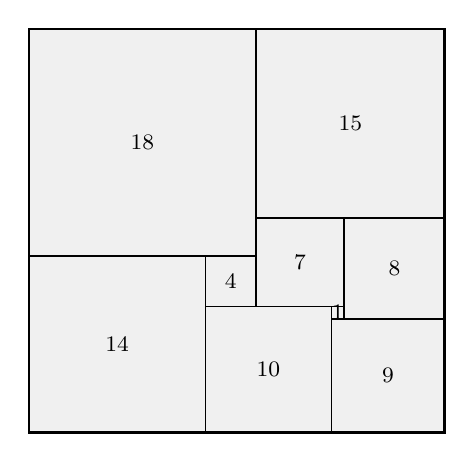
\begin{tikzpicture}[x=0.16cm,y=0.16cm]
\draw[line width=0.5pt,fill=black!6] (0,14) rectangle (18,32);
\node[font=\footnotesize] at (9.0,23.0) {18};
\draw[line width=0.5pt,fill=black!6] (18,17) rectangle (33,32);
\node[font=\footnotesize] at (25.5,24.5) {15};
\draw[line width=0.5pt,fill=black!6] (18,10) rectangle (25,17);
\node[font=\footnotesize] at (21.5,13.5) {7};
\draw[line width=0.5pt,fill=black!6] (25,9) rectangle (33,17);
\node[font=\footnotesize] at (29.0,13.0) {8};
\draw[line width=0.5pt,fill=black!6] (0,0) rectangle (14,14);
\node[font=\footnotesize] at (7.0,7.0) {14};
\draw[line width=0.5pt,fill=black!6] (14,10) rectangle (18,14);
\node[font=\footnotesize] at (16.0,12.0) {4};
\draw[line width=0.5pt,fill=black!6] (14,0) rectangle (24,10);
\node[font=\footnotesize] at (19.0,5.0) {10};
\draw[line width=0.5pt,fill=black!6] (24,9) rectangle (25,10);
\node[font=\footnotesize] at (24.5,9.5) {1};
\draw[line width=0.5pt,fill=black!6] (24,0) rectangle (33,9);
\node[font=\footnotesize] at (28.5,4.5) {9};
\draw[line width=1pt] (0,0) rectangle (33,32);
\end{tikzpicture}\qquad
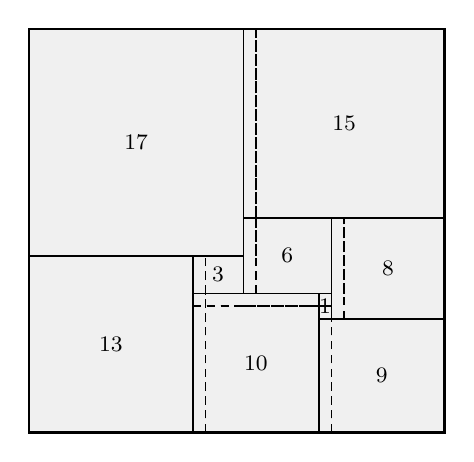
\begin{tikzpicture}[x=0.16cm,y=0.16cm]
\draw[line width=0.5pt,fill=black!6] (0,14) rectangle (17,32);
\node[font=\footnotesize] at (8.5,23.0) {17};
\draw[line width=0.5pt,fill=black!6] (17,17) rectangle (33,32);
\node[font=\footnotesize] at (25.0,24.5) {15};
\draw[line width=0.5pt,fill=black!6] (17,11) rectangle (24,17);
\node[font=\footnotesize] at (20.5,14.0) {6};
\draw[line width=0.5pt,fill=black!6] (24,9) rectangle (33,17);
\node[font=\footnotesize] at (28.5,13.0) {8};
\draw[line width=0.5pt,fill=black!6] (0,0) rectangle (13,14);
\node[font=\footnotesize] at (6.5,7.0) {13};
\draw[line width=0.5pt,fill=black!6] (13,11) rectangle (17,14);
\node[font=\footnotesize] at (15.0,12.5) {3};
\draw[line width=0.5pt,fill=black!6] (13,0) rectangle (23,11);
\node[font=\footnotesize] at (18.0,5.5) {10};
\draw[line width=0.5pt,fill=black!6] (23,9) rectangle (24,11);
\node[font=\footnotesize] at (23.5,10.0) {1};
\draw[line width=0.5pt,fill=black!6] (23,0) rectangle (33,9);
\node[font=\footnotesize] at (28.0,4.5) {9};
\draw[line width=1pt] (0,0) rectangle (33,32);
\draw[densely dashed, line width=0.6pt] (18,14) -- (18,32);
\draw[densely dashed, line width=0.6pt] (18,17) -- (18,32);
\draw[densely dashed, line width=0.6pt] (18,11) -- (18,17);
\draw[densely dashed, line width=0.6pt] (25,11) -- (25,17);
\draw[densely dashed, line width=0.6pt] (17,10) -- (24,10);
\draw[densely dashed, line width=0.6pt] (25,9) -- (25,17);
\draw[densely dashed, line width=0.6pt] (14,0) -- (14,14);
\draw[densely dashed, line width=0.6pt] (14,11) -- (14,14);
\draw[densely dashed, line width=0.6pt] (18,11) -- (18,14);
\draw[densely dashed, line width=0.6pt] (13,10) -- (17,10);
\draw[densely dashed, line width=0.6pt] (14,0) -- (14,11);
\draw[densely dashed, line width=0.6pt] (24,0) -- (24,11);
\draw[densely dashed, line width=0.6pt] (13,10) -- (23,10);
\draw[densely dashed, line width=0.6pt] (24,9) -- (24,11);
\draw[densely dashed, line width=0.6pt] (25,9) -- (25,11);
\draw[densely dashed, line width=0.6pt] (23,10) -- (24,10);
\draw[densely dashed, line width=0.6pt] (24,0) -- (24,9);
\end{tikzpicture}

\caption{Left: Moro\'n's $33\times32$ rectangle cut into nine distinct squares, labelled by side.
Right: the vertical cut lines at $x=14,18,24,25$ move one unit left and the horizontal line at
$y=10$ moves one unit up (old positions dashed). Every square becomes an almost-square, labelled
by size.}
\label{fig:moron}
\end{figure}

One tiling settles one $n$. To settle infinitely many we want to scale the picture, and here the
rectangle lets us down: scaled by $t$, Moro\'n's rectangle becomes $33t\times32t$, which is no longer
an almost-square. A square has no such problem. Scale a squared square by $t$ and move its cut lines
so that every piece, the outer square included, gains one unit more in one direction than in the
other. This works at every scale at once, and Sections~\ref{sec:inflation} and~\ref{sec:parity}
turn it into a proof.

The question comes from Erich Friedman's Problem of the Month for May
2012~\cite{friedman-0512}. Solvers found tilings for every $n$ from $20$ to $55$ and for
$n=10,12,14,15,18$; Friedman's list of unsolved problems from the column then recorded the
conjecture that every $n\ge20$ works~\cite{friedman-unsolved}.

A neighbouring problem uses every size from $1$ to $m$ at once. The almost-square packing problem asks
for the rectangle of least area into which $1\times2,2\times3,\dots,m\times(m+1)$ fit without overlap;
Simonis and O'Sullivan~\cite{simonis} solved it by computer up to $m=26$, and Ellard and
MacHale~\cite{ellard} study packings of such rectangles. When the frame must itself be
an almost-square, the area condition holds only for $m=1,3,8,20,34$, and exact fits are known for each
of them, the last found by van den Berg, Braam, Moes, Suilen and Bhulai~\cite{vdberg}. For $m>1$ these
fits are tilings in our sense, of the almost-squares of sizes $4$, $15$, $55$ and $119$. Allowing any
set of distinct sizes, as Friedman does, is what makes every large $n$ reachable.

\begin{thm}\label{thm:main}
The $n\times(n+1)$ almost-square can be cut into almost-squares of distinct sizes smaller than $n$
if and only if $n\in\{4,10,12,14,15,18\}$ or $n\ge20$.
\end{thm}

The new parts are a construction for every $n\ge56$, where the only earlier case we know of is $n=119$,
and the impossibility for every $n\le19$ outside the list. The proof has three steps. Section~\ref{sec:inflation} shows that moving cut lines preserves a
dissection, using one counting identity, and that one good set of moves works for all large scales.
Section~\ref{sec:parity} uses the same identity to explain which squared squares can be inflated
and which values of $n$ they reach. Section~\ref{sec:proof} supplies the finite data for large $n$,
and Section~\ref{sec:small} settles $n\le19$. Section~\ref{sec:verify} describes how the finite
checks were verified.

\begin{figure}[ht]
\centering
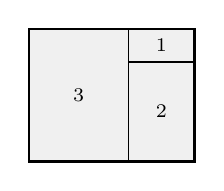
\begin{tikzpicture}[x=0.42cm,y=0.42cm]
\draw[line width=0.5pt,fill=black!6] (0,0) rectangle (3,4);
\node[font=\scriptsize] at (1.5,2.0) {3};
\draw[line width=0.5pt,fill=black!6] (3,0) rectangle (5,3);
\node[font=\scriptsize] at (4.0,1.5) {2};
\draw[line width=0.5pt,fill=black!6] (3,3) rectangle (5,4);
\node[font=\scriptsize] at (4.0,3.5) {1};
\draw[line width=1pt] (0,0) rectangle (5,4);
\end{tikzpicture}\qquad
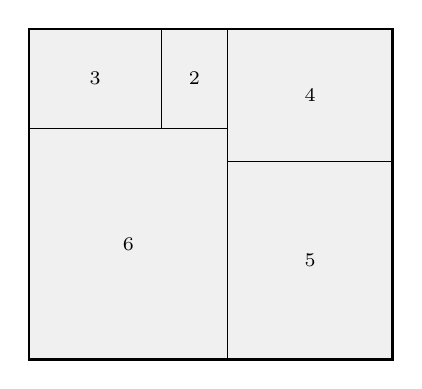
\begin{tikzpicture}[x=0.42cm,y=0.42cm]
\draw[line width=0.5pt,fill=black!6] (0,0) rectangle (6,7);
\node[font=\scriptsize] at (3.0,3.5) {6};
\draw[line width=0.5pt,fill=black!6] (6,0) rectangle (11,6);
\node[font=\scriptsize] at (8.5,3.0) {5};
\draw[line width=0.5pt,fill=black!6] (6,6) rectangle (11,10);
\node[font=\scriptsize] at (8.5,8.0) {4};
\draw[line width=0.5pt,fill=black!6] (0,7) rectangle (4,10);
\node[font=\scriptsize] at (2.0,8.5) {3};
\draw[line width=0.5pt,fill=black!6] (4,7) rectangle (6,10);
\node[font=\scriptsize] at (5.0,8.5) {2};
\draw[line width=1pt] (0,0) rectangle (11,10);
\end{tikzpicture}

\caption{Tilings of the $5\times4$ almost-square by sizes $1,2,3$ and of the $11\times10$ almost-square
by sizes $2,\dots,6$, labelled by size.}
\label{fig:small}
\end{figure}

\section{Moving cut lines}\label{sec:inflation}

Throughout, coordinates, side lengths, scales and shifts are integers; Lemma~\ref{lem:integer}
below shows that nothing is lost by this. Write $\R_n$ for the rectangle $[0,n+1]\times[0,n]$, the
almost-square to be tiled, and call a tiling of $\R_n$ \emph{admissible} if its tiles are
almost-squares of distinct sizes, all smaller than $n$.

\subsection*{Shifts} Table~\ref{tab:moron} records Moro\'n's example square by square. The vertical
cut lines are at $x\in\{0,14,18,24,25,33\}$ and the horizontal ones at $y\in\{0,9,10,14,17,32\}$. The
moves are $u(14)=u(18)=u(24)=u(25)=-1$ and $v(10)=1$, every other line staying put. The $10$-square
has left side at $x=14$ and right side at $x=24$, both moved by $-1$, so its width does not change;
its bottom at $y=0$ stays and its top at $y=10$ rises by one, so it becomes $10\times11$.

\begin{table}[ht]
\caption{Moro\'n's squares under the moves of Figure~\ref{fig:moron}. Each square is given by its
side $s$ and lower-left corner $(x,y)$; $\delta u$ and $\delta v$ are the changes in its width and
height. The last column is $\varepsilon=\delta u-\delta v$.}
\label{tab:moron}
\centering\small
\begin{tabular}{rcrrcrr}
\toprule
$s$ & $(x,y)$ & $\delta u$ & $\delta v$ & new shape & size & $\varepsilon$\\
\midrule
18 & $(0,14)$ & $-1$ & $0$ & $17\times18$ & 17 & $-1$\\
15 & $(18,17)$ & $1$ & $0$ & $16\times15$ & 15 & $1$\\
14 & $(0,0)$ & $-1$ & $0$ & $13\times14$ & 13 & $-1$\\
10 & $(14,0)$ & $0$ & $1$ & $10\times11$ & 10 & $-1$\\
9 & $(24,0)$ & $1$ & $0$ & $10\times9$ & 9 & $1$\\
8 & $(25,9)$ & $1$ & $0$ & $9\times8$ & 8 & $1$\\
7 & $(18,10)$ & $0$ & $-1$ & $7\times6$ & 6 & $1$\\
4 & $(14,10)$ & $0$ & $-1$ & $4\times3$ & 3 & $1$\\
1 & $(24,9)$ & $0$ & $1$ & $1\times2$ & 1 & $-1$\\
\bottomrule
\end{tabular}
\end{table}

In general, let $Q=[0,W]\times[0,H]$ be dissected into squares $Q_i=[x_i,x_i+s_i]\times[y_i,y_i+s_i]$,
$1\le i\le m$. Let $\mathcal X$ be the set of $x$-coordinates of vertical sides of the squares and
$\mathcal Y$ the set of $y$-coordinates of horizontal sides. A \emph{shift} is a pair of integer
functions $u$ on $\mathcal X$ and $v$ on $\mathcal Y$ with $u(0)=v(0)=0$. At scale $t\ge1$, put
\[
X_t(a)=ta+u(a),\qquad Y_t(b)=tb+v(b),
\]
so that $X_t$ places each vertical cut line at $t$ times its old position plus its shift, and $Y_t$
does the same for horizontal lines. Square $i$ becomes the rectangle
\[
Q_i^t=[X_t(x_i),X_t(x_i+s_i)]\times[Y_t(y_i),Y_t(y_i+s_i)],
\]
of width $ts_i+\delta u_i$ and height $ts_i+\delta v_i$, where
$\delta u_i=u(x_i+s_i)-u(x_i)$ and $\delta v_i=v(y_i+s_i)-v(y_i)$ are the columns of
Table~\ref{tab:moron}. It is an almost-square exactly when $\delta u_i-\delta v_i=\pm1$
(Figure~\ref{fig:shift}).

\begin{figure}[ht]
\centering
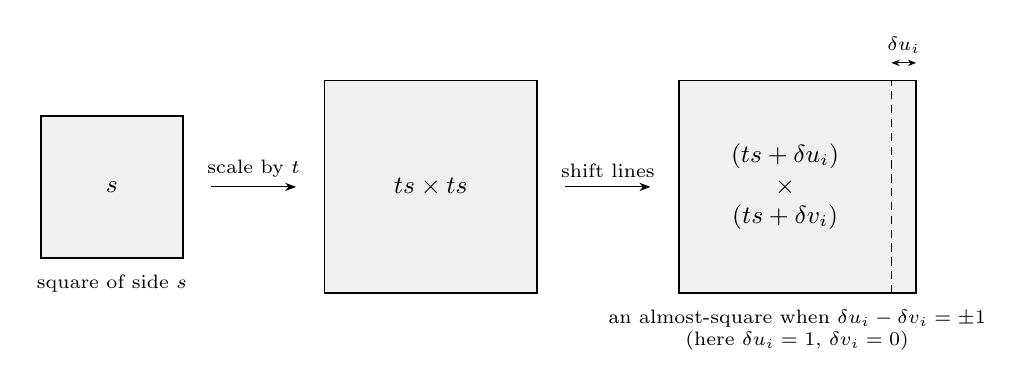
\begin{tikzpicture}[scale=0.9]
\draw[line width=0.6pt, fill=black!6] (0,0) rectangle (2,2);
\node[font=\small] at (1,1) {$s$};
\node[font=\scriptsize, below] at (1,-0.1) {square of side $s$};
\draw[-{Stealth[length=4pt]}] (2.4,1) -- node[above, font=\scriptsize] {scale by $t$} (3.6,1);
\draw[line width=0.6pt, fill=black!6] (4,-0.5) rectangle (7,2.5);
\node[font=\small] at (5.5,1) {$ts\times ts$};
\draw[-{Stealth[length=4pt]}] (7.4,1) -- node[above, font=\scriptsize] {shift lines} (8.6,1);
\draw[line width=0.6pt, fill=black!6] (9,-0.5) rectangle (12.35,2.5);
\draw[line width=0.4pt, densely dashed] (12,-0.5) -- (12,2.5);
\draw[{Stealth[length=3pt]}-{Stealth[length=3pt]}] (12,2.75) -- node[above, font=\scriptsize] {$\delta u_i$} (12.35,2.75);
\node[font=\small, align=center] at (10.5,1) {$(ts+\delta u_i)$\\$\times$\\$(ts+\delta v_i)$};
\node[font=\scriptsize, below, align=center] at (10.67,-0.6) {an almost-square when $\delta u_i-\delta v_i=\pm1$\\(here $\delta u_i=1$, $\delta v_i=0$)};
\end{tikzpicture}
\caption{What a shift does to one square. After scaling, the cut lines around it move by small
integers, changing its width by $\delta u_i$ and its height by $\delta v_i$.}
\label{fig:shift}
\end{figure}

\subsection*{Why the pieces still fit} Moving lines could, in principle, make pieces overlap or leave
gaps. Overlaps are easy to rule out: two squares of the dissection lie on opposite sides of some
cut line, and if the lines keep their order they stay on opposite sides. Gaps need a count, and
the count we need is worth stating on its own, because Section~\ref{sec:parity} uses it twice more.

For Moro\'n's rectangle, take any function $f$ on the vertical cut lines and any $g$ on the
horizontal ones. Each square contributes the product of how much $f$ changes across it and how much
$g$ changes across it. With $f(x)=x$ and $g(y)=y$ the contributions are the areas $s_i^2$, and their
sum is the area $33\cdot32$ of the rectangle. More surprisingly, take $f=u$ and $g(y)=y$. The contributions
are $\delta u_i\,s_i$, which from Table~\ref{tab:moron} are $-18,15,-14,0,9,8,0,0,0$. They add up to
$0$, and so does the same quantity for the whole rectangle, $u(33)\cdot32$. The next lemma says this
always happens, for every $f$ and $g$.

\begin{figure}[ht]
\centering
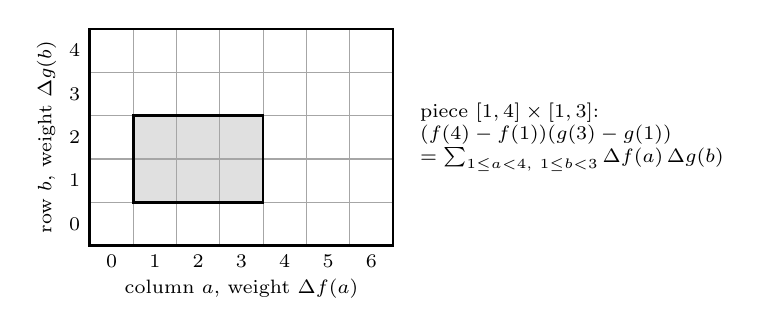
\begin{tikzpicture}[scale=0.55]
\fill[black!12] (1,1) rectangle (4,3);
\draw[black!35] (0,0) grid (7,5);
\draw[line width=1pt] (0,0) rectangle (7,5);
\draw[line width=1pt] (1,1) rectangle (4,3);
\foreach \a in {0,...,6} {\node[font=\scriptsize, below] at (\a+0.5,0) {$\a$};}
\foreach \b in {0,...,4} {\node[font=\scriptsize, left] at (0,\b+0.5) {$\b$};}
\node[font=\scriptsize, below] at (3.5,-0.55) {column $a$, weight $\Delta f(a)$};
\node[font=\scriptsize, rotate=90, above] at (-0.55,2.5) {row $b$, weight $\Delta g(b)$};
\node[font=\scriptsize, align=left, right] at (7.4,2.5) {piece $[1,4]\times[1,3]$:\\
$(f(4)-f(1))(g(3)-g(1))$\\$=\sum_{1\le a<4,\ 1\le b<3}\Delta f(a)\,\Delta g(b)$};
\end{tikzpicture}
\caption{The proof of Lemma~\ref{lem:balance}. Give the unit cell in column $a$ and row $b$ the
weight $\Delta f(a)\,\Delta g(b)$. A piece's term is the total weight of its cells, and every cell lies in
exactly one piece.}
\label{fig:balance}
\end{figure}

\begin{lem}[Balance]\label{lem:balance}
Let $[0,W]\times[0,H]$ be dissected into rectangles $[l_i,r_i]\times[b_i,t_i]$ with integer
corners, and let $f,g$ be integer functions on the integers. (A function given only on the cut
lines can be extended to all integers in any way; only its values on the cut lines matter.) Then
\[
\sum_i\bigl(f(r_i)-f(l_i)\bigr)\bigl(g(t_i)-g(b_i)\bigr)=\bigl(f(W)-f(0)\bigr)\bigl(g(H)-g(0)\bigr).
\]
\end{lem}

\noindent
The left side adds, over the pieces, the change of $f$ across the piece times the change of $g$ up
it; the right side is the same quantity for the whole rectangle.

\begin{proof}
Write $\Delta f(a)=f(a+1)-f(a)$. The change of $f$ across $[l,r]$ is $\sum_{l\le a<r}\Delta f(a)$, so
the term for piece $i$ is the sum of $\Delta f(a)\,\Delta g(b)$ over the unit cells
$[a,a+1]\times[b,b+1]$ of that piece. Every unit cell of $[0,W]\times[0,H]$ lies in exactly one piece,
so the left side is the sum of $\Delta f(a)\,\Delta g(b)$ over all unit cells, which factorises as the
right side (Figure~\ref{fig:balance}).
\end{proof}

\begin{lem}[Inflation]\label{lem:inflation}
Suppose $X_t$ is strictly increasing on $\mathcal X$ and $Y_t$ is strictly increasing on
$\mathcal Y$. Then the rectangles $Q_i^t$ tile $[0,X_t(W)]\times[0,Y_t(H)]$. If moreover
$\delta u_i-\delta v_i=\pm1$ for every $i$, then $Q_i^t$ is an almost-square of size
$ts_i+\min(\delta u_i,\delta v_i)$.
\end{lem}

\begin{proof}
Two distinct squares of the dissection have disjoint interiors, so one lies entirely to the left of,
or entirely below, the other; say $x_i+s_i\le x_j$. Since $X_t$ is increasing,
$X_t(x_i+s_i)\le X_t(x_j)$, and $Q_i^t$ and $Q_j^t$ do not overlap. Each $Q_i^t$ lies in the big
rectangle because $X_t(0)=0$ and $X_t$ is increasing, and likewise for $Y_t$. Lemma~\ref{lem:balance}
with $f=X_t$ and $g=Y_t$ says that the areas of the $Q_i^t$ add up to $X_t(W)\,Y_t(H)$, the area of
the big rectangle. Non-overlapping rectangles inside it with the full total area cover every unit cell
exactly once, so they tile it. The last sentence is the shape computation above.
\end{proof}

\subsection*{Squares, and every scale at once} When $W=H=S$, the big rectangle is
$(tS+u(S))\times(tS+v(S))$. It is an almost-square at every scale exactly when $u(S)-v(S)=\pm1$; we
take $u(S)-v(S)=1$, which a reflection in the diagonal arranges. Call a shift with
$\delta u_i-\delta v_i=\pm1$ for every square and $u(S)-v(S)=1$ an \emph{inflation}. It turns the
squared square into $\R_n$ with $n=tS+v(S)$, whose pieces have sizes $ts_i+c_i$ with
$c_i=\min(\delta u_i,\delta v_i)$. Moro\'n's rectangle needed $W-H=1$ to begin with, and could
not be scaled; a squared square gets its extra unit from the shift.

Our main example is the inflation of Duijvestijn's squared square of side $112$ that is zero except
for the values
\[
u:\ \inflU
\]
and
\[
v:\ \inflV.
\]
Here $v(112)=0$, so this inflation gives $n=112t$. The $50$-square in the upper-left corner has
$\delta u=0$ and $\delta v=v(112)-v(62)=1$; at $t=2$ it becomes $100\times101$, the almost-square of
size $100$. Every $c_i$ is $0$ or $-1$. At $t=1$ two sizes clash: the $16$-square has $c=-1$ and
the $15$-square has $c=0$, giving sizes $16t-1$ and $15t$, which agree only at $t=1$. From $t=2$ on
the $21$ sizes are distinct, and Figure~\ref{fig:inflate} shows the tiling of $\R_{224}$.

\begin{figure}[ht]
\centering
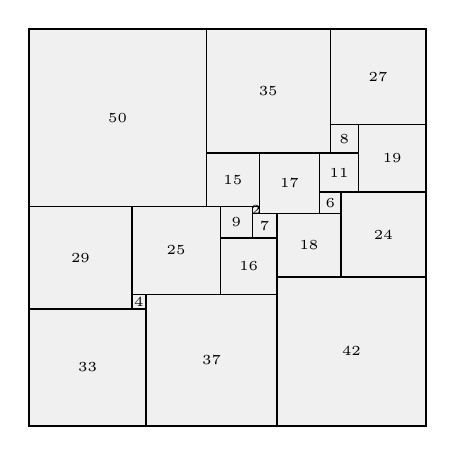
\begin{tikzpicture}[x=0.045cm,y=0.045cm]
\draw[line width=0.5pt,fill=black!6] (0,62) rectangle (50,112);
\node[font=\tiny] at (25.0,87.0) {50};
\draw[line width=0.5pt,fill=black!6] (50,77) rectangle (85,112);
\node[font=\tiny] at (67.5,94.5) {35};
\draw[line width=0.5pt,fill=black!6] (85,85) rectangle (112,112);
\node[font=\tiny] at (98.5,98.5) {27};
\draw[line width=0.5pt,fill=black!6] (85,77) rectangle (93,85);
\node[font=\tiny] at (89.0,81.0) {8};
\draw[line width=0.5pt,fill=black!6] (93,66) rectangle (112,85);
\node[font=\tiny] at (102.5,75.5) {19};
\draw[line width=0.5pt,fill=black!6] (50,62) rectangle (65,77);
\node[font=\tiny] at (57.5,69.5) {15};
\draw[line width=0.5pt,fill=black!6] (65,60) rectangle (82,77);
\node[font=\tiny] at (73.5,68.5) {17};
\draw[line width=0.5pt,fill=black!6] (82,66) rectangle (93,77);
\node[font=\tiny] at (87.5,71.5) {11};
\draw[line width=0.5pt,fill=black!6] (82,60) rectangle (88,66);
\node[font=\tiny] at (85.0,63.0) {6};
\draw[line width=0.5pt,fill=black!6] (88,42) rectangle (112,66);
\node[font=\tiny] at (100.0,54.0) {24};
\draw[line width=0.5pt,fill=black!6] (0,33) rectangle (29,62);
\node[font=\tiny] at (14.5,47.5) {29};
\draw[line width=0.5pt,fill=black!6] (29,37) rectangle (54,62);
\node[font=\tiny] at (41.5,49.5) {25};
\draw[line width=0.5pt,fill=black!6] (54,53) rectangle (63,62);
\node[font=\tiny] at (58.5,57.5) {9};
\draw[line width=0.5pt,fill=black!6] (63,60) rectangle (65,62);
\node[font=\tiny] at (64.0,61.0) {2};
\draw[line width=0.5pt,fill=black!6] (63,53) rectangle (70,60);
\node[font=\tiny] at (66.5,56.5) {7};
\draw[line width=0.5pt,fill=black!6] (70,42) rectangle (88,60);
\node[font=\tiny] at (79.0,51.0) {18};
\draw[line width=0.5pt,fill=black!6] (54,37) rectangle (70,53);
\node[font=\tiny] at (62.0,45.0) {16};
\draw[line width=0.5pt,fill=black!6] (70,0) rectangle (112,42);
\node[font=\tiny] at (91.0,21.0) {42};
\draw[line width=0.5pt,fill=black!6] (29,33) rectangle (33,37);
\node[font=\tiny] at (31.0,35.0) {4};
\draw[line width=0.5pt,fill=black!6] (33,0) rectangle (70,37);
\node[font=\tiny] at (51.5,18.5) {37};
\draw[line width=0.5pt,fill=black!6] (0,0) rectangle (33,33);
\node[font=\tiny] at (16.5,16.5) {33};
\draw[line width=1pt] (0,0) rectangle (112,112);
\end{tikzpicture}\qquad
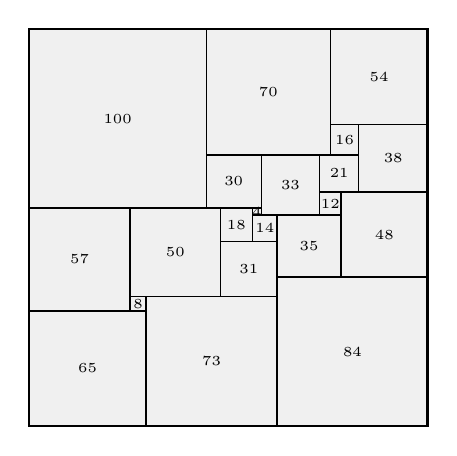
\begin{tikzpicture}[x=0.0225cm,y=0.0225cm]
\draw[line width=0.5pt,fill=black!6] (0,123) rectangle (100,224);
\node[font=\tiny] at (50.0,173.5) {100};
\draw[line width=0.5pt,fill=black!6] (100,153) rectangle (170,224);
\node[font=\tiny] at (135.0,188.5) {70};
\draw[line width=0.5pt,fill=black!6] (170,170) rectangle (225,224);
\node[font=\tiny] at (197.5,197.0) {54};
\draw[line width=0.5pt,fill=black!6] (170,153) rectangle (186,170);
\node[font=\tiny] at (178.0,161.5) {16};
\draw[line width=0.5pt,fill=black!6] (186,132) rectangle (225,170);
\node[font=\tiny] at (205.5,151.0) {38};
\draw[line width=0.5pt,fill=black!6] (100,123) rectangle (131,153);
\node[font=\tiny] at (115.5,138.0) {30};
\draw[line width=0.5pt,fill=black!6] (131,119) rectangle (164,153);
\node[font=\tiny] at (147.5,136.0) {33};
\draw[line width=0.5pt,fill=black!6] (164,132) rectangle (186,153);
\node[font=\tiny] at (175.0,142.5) {21};
\draw[line width=0.5pt,fill=black!6] (164,119) rectangle (176,132);
\node[font=\tiny] at (170.0,125.5) {12};
\draw[line width=0.5pt,fill=black!6] (176,84) rectangle (225,132);
\node[font=\tiny] at (200.5,108.0) {48};
\draw[line width=0.5pt,fill=black!6] (0,65) rectangle (57,123);
\node[font=\tiny] at (28.5,94.0) {57};
\draw[line width=0.5pt,fill=black!6] (57,73) rectangle (108,123);
\node[font=\tiny] at (82.5,98.0) {50};
\draw[line width=0.5pt,fill=black!6] (108,104) rectangle (126,123);
\node[font=\tiny] at (117.0,113.5) {18};
\draw[line width=0.5pt,fill=black!6] (126,119) rectangle (131,123);
\node[font=\tiny] at (128.5,121.0) {4};
\draw[line width=0.5pt,fill=black!6] (126,104) rectangle (140,119);
\node[font=\tiny] at (133.0,111.5) {14};
\draw[line width=0.5pt,fill=black!6] (140,84) rectangle (176,119);
\node[font=\tiny] at (158.0,101.5) {35};
\draw[line width=0.5pt,fill=black!6] (108,73) rectangle (140,104);
\node[font=\tiny] at (124.0,88.5) {31};
\draw[line width=0.5pt,fill=black!6] (140,0) rectangle (225,84);
\node[font=\tiny] at (182.5,42.0) {84};
\draw[line width=0.5pt,fill=black!6] (57,65) rectangle (66,73);
\node[font=\tiny] at (61.5,69.0) {8};
\draw[line width=0.5pt,fill=black!6] (66,0) rectangle (140,73);
\node[font=\tiny] at (103.0,36.5) {73};
\draw[line width=0.5pt,fill=black!6] (0,0) rectangle (66,65);
\node[font=\tiny] at (33.0,32.5) {65};
\draw[line width=1pt] (0,0) rectangle (225,224);
\end{tikzpicture}

\caption{Duijvestijn's squared square of side $112$ and its inflation at $t=2$, an admissible tiling
of $\R_{224}$ by $21$ almost-squares. Three vertical and six horizontal cut lines have moved, by at
most two units.}
\label{fig:inflate}
\end{figure}

The clash is the only thing that can go wrong for large $t$, and it can go wrong at most once for
each pair of squares.

\begin{lem}[All large scales]\label{lem:scales}
Let $u,v$ be an inflation of a squared square of side $S$ whose squares have distinct sides, and put
$n(t)=tS+v(S)$. Let $t_0$ be the least positive integer that exceeds every integer collision point
$(c_j-c_i)/(s_i-s_j)$ and at which every consecutive gap $t(a'-a)+u(a')-u(a)$ and
$t(b'-b)+v(b')-v(b)$, every size $ts_i+c_i$ and every difference $n(t)-(ts_i+c_i)$ is positive. Then
for every $t\ge t_0$, Lemma~\ref{lem:inflation} gives an admissible tiling of $\R_{n(t)}$.
\end{lem}

\begin{proof}
Each quantity listed is an affine function of $t$ with positive slope, so once positive it stays
positive. Two sizes $ts_i+c_i$ and $ts_j+c_j$ with $s_i\ne s_j$ agree for at most one $t$, the
collision point. For $t\ge t_0$ the cut lines keep their order, every tile is an almost-square of
positive size less than $n(t)$, and the sizes are distinct.
\end{proof}

\section{Which squared squares inflate}\label{sec:parity}

The example above reaches $n=112t$. Can some other inflation of the same square reach an odd $n$?
That needs $v(112)$ odd, and the answer is no, for a reason that can be seen in six squares.

Figure~\ref{fig:parity} shades a stack of six squares of the $112$-square, of sides $42,18,6,11,8,27$
from the bottom edge to the top edge. Each square's top is the next square's bottom, so the height
changes along the stack telescope: $\sum\delta v_i=v(112)-v(0)=v(112)$. The widths behave
differently. The squares run between $x=70$ and $112$, $70$ and $88$, $82$ and $88$, $82$ and $93$,
$85$ and $93$, and $85$ and $112$, so
\[
\sum\delta u_i=2\bigl(u(112)+u(88)+u(93)-u(70)-u(82)-u(85)\bigr),
\]
an even number. Now each $\varepsilon_i=\delta u_i-\delta v_i$ is $\pm1$, and a sum of six odd numbers
is even. Hence $v(112)=\sum\delta u_i-\sum\varepsilon_i$ is even, for every inflation. In the example
the $\varepsilon_i$ are $1,1,-1,1,-1,1$, $\sum\delta u_i=2$ and $v(112)=0$.

\begin{figure}[ht]
\centering
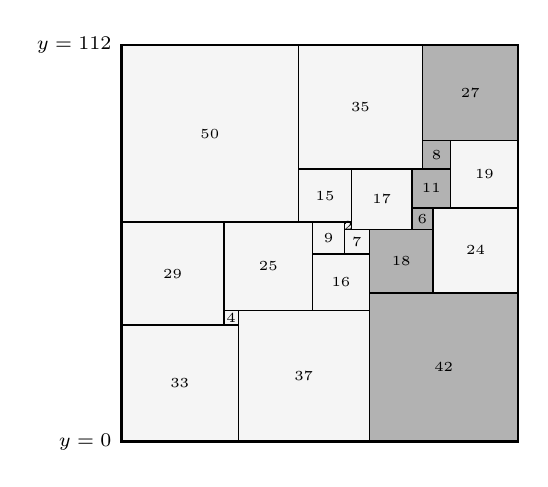
\begin{tikzpicture}[x=0.045cm,y=0.045cm]
\draw[line width=0.5pt,fill=black!4] (0,62) rectangle (50,112);
\node[font=\tiny] at (25.0,87.0) {50};
\draw[line width=0.5pt,fill=black!4] (50,77) rectangle (85,112);
\node[font=\tiny] at (67.5,94.5) {35};
\draw[line width=0.5pt,fill=black!30] (85,85) rectangle (112,112);
\node[font=\tiny] at (98.5,98.5) {27};
\draw[line width=0.5pt,fill=black!30] (85,77) rectangle (93,85);
\node[font=\tiny] at (89.0,81.0) {8};
\draw[line width=0.5pt,fill=black!4] (93,66) rectangle (112,85);
\node[font=\tiny] at (102.5,75.5) {19};
\draw[line width=0.5pt,fill=black!4] (50,62) rectangle (65,77);
\node[font=\tiny] at (57.5,69.5) {15};
\draw[line width=0.5pt,fill=black!4] (65,60) rectangle (82,77);
\node[font=\tiny] at (73.5,68.5) {17};
\draw[line width=0.5pt,fill=black!30] (82,66) rectangle (93,77);
\node[font=\tiny] at (87.5,71.5) {11};
\draw[line width=0.5pt,fill=black!30] (82,60) rectangle (88,66);
\node[font=\tiny] at (85.0,63.0) {6};
\draw[line width=0.5pt,fill=black!4] (88,42) rectangle (112,66);
\node[font=\tiny] at (100.0,54.0) {24};
\draw[line width=0.5pt,fill=black!4] (0,33) rectangle (29,62);
\node[font=\tiny] at (14.5,47.5) {29};
\draw[line width=0.5pt,fill=black!4] (29,37) rectangle (54,62);
\node[font=\tiny] at (41.5,49.5) {25};
\draw[line width=0.5pt,fill=black!4] (54,53) rectangle (63,62);
\node[font=\tiny] at (58.5,57.5) {9};
\draw[line width=0.5pt,fill=black!4] (63,60) rectangle (65,62);
\node[font=\tiny] at (64.0,61.0) {2};
\draw[line width=0.5pt,fill=black!4] (63,53) rectangle (70,60);
\node[font=\tiny] at (66.5,56.5) {7};
\draw[line width=0.5pt,fill=black!30] (70,42) rectangle (88,60);
\node[font=\tiny] at (79.0,51.0) {18};
\draw[line width=0.5pt,fill=black!4] (54,37) rectangle (70,53);
\node[font=\tiny] at (62.0,45.0) {16};
\draw[line width=0.5pt,fill=black!30] (70,0) rectangle (112,42);
\node[font=\tiny] at (91.0,21.0) {42};
\draw[line width=0.5pt,fill=black!4] (29,33) rectangle (33,37);
\node[font=\tiny] at (31.0,35.0) {4};
\draw[line width=0.5pt,fill=black!4] (33,0) rectangle (70,37);
\node[font=\tiny] at (51.5,18.5) {37};
\draw[line width=0.5pt,fill=black!4] (0,0) rectangle (33,33);
\node[font=\tiny] at (16.5,16.5) {33};
\draw[line width=1pt] (0,0) rectangle (112,112);
\node[font=\scriptsize, left] at (0,0) {$y=0$};
\node[font=\scriptsize, left] at (0,112) {$y=112$};
\end{tikzpicture}

\caption{Six squares of Duijvestijn's square stacked from bottom to top. Each interior horizontal line
between them is the top of one and the bottom of the next, and each of $x=70,82,85,88,93,112$ is a
vertical side exactly twice. Only $y=0$ and $y=112$ occur once.}
\label{fig:parity}
\end{figure}

Nothing in this argument used the stack shape. It used only that each $x$-coordinate occurs an even
number of times among the vertical sides of the chosen squares, and each $y$-coordinate among their
horizontal sides, apart from the two we wanted to learn about.

\begin{lem}[Parity]\label{lem:parity}
Let $u,v$ be a shift with $\delta u_i-\delta v_i=\pm1$ for all $i$, and let $T$ be a set of squares. Then
\[
\sum_{i\in T}\bigl(u(x_i)+u(x_i+s_i)+v(y_i)+v(y_i+s_i)\bigr)\equiv|T|\pmod 2 .
\]
In particular, if every $x$-coordinate occurs an even number of times among the vertical sides of the
squares in $T$, and every $y$-coordinate among their horizontal sides, then $|T|$ is even.
\end{lem}

\begin{proof}
For each $i$, $\delta u_i-\delta v_i$ is odd and is congruent to $u(x_i)+u(x_i+s_i)+v(y_i)+v(y_i+s_i)$
modulo $2$, because $-1\equiv1$. Sum over $T$. If every coordinate occurs an even number of times,
every shift value appears an even number of times on the left, so the left side is even.
\end{proof}

Squared squares are named below by their Bouwkamp codes, as listed by Moews~\cite{moews}; each square
is written $(s;x,y)$ with lower-left corner $(x,y)$. The square of side $112$ is Duijvestijn's, of
order $21$, the lowest possible~\cite{duij78}. Squares of side $110$ were found by
Duijvestijn~\cite{duij93}, and Gambini showed that $110$ is the smallest side of any perfect
squared square~\cite{gambini}.

\begin{prop}\label{prop:three}\leavevmode
\begin{enumerate}
\item Every inflation of Duijvestijn's square of side $112$, code $(50,35,27)(8,19)\dots$, has
$v(112)$ even.
\item Every inflation of the order-$22$ square of side $110$ with code $(60,50)(27,23)\dots$ has
$v(110)$ odd.
\item The order-$22$ square of side $139$ with code $(80,59)(21,38)\dots$ has no inflation.
\end{enumerate}
\end{prop}

\begin{proof}
Apply Lemma~\ref{lem:parity} with the following sets.

(1) Take the stack of Figure~\ref{fig:parity},
\[
T=\{(42;70,0),(18;70,42),(6;82,60),(11;82,66),(8;85,77),(27;85,85)\}.
\]
Every coordinate occurs an even number of times except $y=0$ and $y=112$, so
$v(0)+v(112)\equiv6\equiv0$.

(2) Take
\[
\begin{aligned}
T=\{&(26;0,0),(22;24,28),(18;92,0),(16;75,17),(14;46,36),\\
&(12;63,21),(9;54,21),(6;54,30),(2;24,26),(1;91,17)\}.
\end{aligned}
\]
Every coordinate occurs an even number of times except $x=0$ and $x=110$, so $u(110)\equiv10\equiv0$,
and $v(110)=u(110)-1$ is odd.

(3) Take
\[
\begin{aligned}
T=\{&(80;0,59),(59;80,80),(38;101,42),(32;61,0),(30;0,0),(28;29,31),(24;93,0),\\
&(22;117,0),(20;119,22),(18;101,24),(7;57,35),(3;61,32),(1;29,30)\}.
\end{aligned}
\]
It has thirteen squares and every coordinate occurs an even number of times, so $13$ would be even.
\end{proof}

\subsection*{The signed identity} Lemma~\ref{lem:balance} says more. In Moro\'n's example the
$\varepsilon$ column of Table~\ref{tab:moron} splits the sides into $18+14+10+1=43$ and
$15+9+8+7+4=43$, two equal halves. For the side-$112$ inflation the split is $273$ against
$161$, which differ by $112$.

\begin{cor}\label{cor:signed}
For a shift of a dissection of $[0,W]\times[0,H]$ into squares,
$\sum_i\delta u_i\,s_i=H\,u(W)$ and $\sum_i\delta v_i\,s_i=W\,v(H)$. For an inflation of a squared
square of side $S$, with $\varepsilon_i=\delta u_i-\delta v_i$,
\[
\sum_i\varepsilon_i\,s_i=S.
\]
\end{cor}

\begin{proof}
Lemma~\ref{lem:balance} with $f=u$, $g(y)=y$ gives the first identity, and with $f(x)=x$, $g=v$ the
second. Subtract, with $W=H=S$ and $u(S)-v(S)=1$.
\end{proof}

So an inflation chooses, for each square, which way round its almost-square lies, in such a way that
the signed sides add up to $S$. In Moro\'n's example $W=33$, $H=32$ and $u(33)=v(32)=0$, and both
identities give $0$. This is the electrical balance of Brooks, Smith, Stone and Tutte~\cite{bsst} in
another guise: along any cut line, the squares on either side have the same total length.

\section{Large \texorpdfstring{$n$}{n}}\label{sec:proof}

Let $\Sigma_{112}$ and $\Sigma_{110}$ be the squares of Proposition~\ref{prop:three}(1) and (2). For
each even residue $r$ modulo $112$ there is an inflation of $\Sigma_{112}$ with $v(112)\equiv r$, and for
each odd residue $r$ modulo $110$ an inflation of $\Sigma_{110}$ with $v(110)\equiv r$; the example of
Section~\ref{sec:inflation} is the class $r=0$. That makes $56+55=111$ inflations, one per class, found
by a constraint solver and listed in the ancillary data with their thresholds $t_0$ from
Lemma~\ref{lem:scales}. Each of these $111$ has threshold at most $3$ and reaches its first $n$ by
$360$; two of the spares have $t_0=4$. By Lemma~\ref{lem:scales}, every $n=tS+v(S)$ with $t\ge t_0$ has an admissible tiling.
Proposition~\ref{prop:three} shows that the parities cannot be swapped between the two squares.

These classes leave exactly $151$ values of $n$ with $20\le n\le248$ uncovered, and every $n\ge249$ is
covered. For each uncovered $n$ the data contain an explicit admissible tiling. Those with $n\le45$
came from a direct search. The rest came from Lemma~\ref{lem:inflation} at a fixed scale $t\le3$,
applied to perfect squared rectangles from Moews's catalogue of orders up to $16$~\cite{moews} whose
sides are nearly equal: a scaled rectangle $tW\times tH$ with $tW-tH$ small can still be shifted to an
almost-square at that one scale. Moro\'n's rectangle gives $n=60$ and $n=98$ at $t=2$ and $t=3$ this way,
and a single $57\times55$ rectangle of order $10$ gives $67$ of the $151$ cases at $t=1$. At one fixed
scale the shifts need not be small, only order-preserving: for $n=99$ the outer sides of the rectangle
move by more than $40$ units, and different shifts of the same rectangle reach different $n$.
Figure~\ref{fig:cover} shows how the range $20\le n<260$ is shared out.

\begin{figure}[ht]
\centering
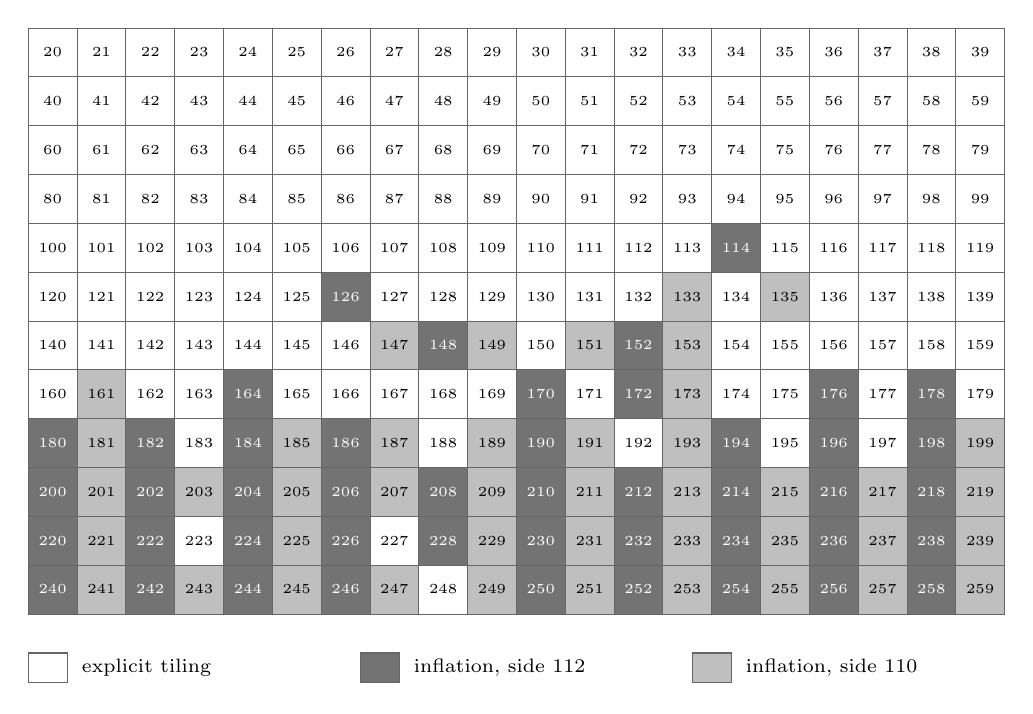
\begin{tikzpicture}[x=0.62cm,y=0.62cm]
\draw[fill=white, draw=black!60, line width=0.3pt] (0,0) rectangle (1,1);
\node[font=\tiny, text=black] at (0.5,0.5) {20};
\draw[fill=white, draw=black!60, line width=0.3pt] (1,0) rectangle (2,1);
\node[font=\tiny, text=black] at (1.5,0.5) {21};
\draw[fill=white, draw=black!60, line width=0.3pt] (2,0) rectangle (3,1);
\node[font=\tiny, text=black] at (2.5,0.5) {22};
\draw[fill=white, draw=black!60, line width=0.3pt] (3,0) rectangle (4,1);
\node[font=\tiny, text=black] at (3.5,0.5) {23};
\draw[fill=white, draw=black!60, line width=0.3pt] (4,0) rectangle (5,1);
\node[font=\tiny, text=black] at (4.5,0.5) {24};
\draw[fill=white, draw=black!60, line width=0.3pt] (5,0) rectangle (6,1);
\node[font=\tiny, text=black] at (5.5,0.5) {25};
\draw[fill=white, draw=black!60, line width=0.3pt] (6,0) rectangle (7,1);
\node[font=\tiny, text=black] at (6.5,0.5) {26};
\draw[fill=white, draw=black!60, line width=0.3pt] (7,0) rectangle (8,1);
\node[font=\tiny, text=black] at (7.5,0.5) {27};
\draw[fill=white, draw=black!60, line width=0.3pt] (8,0) rectangle (9,1);
\node[font=\tiny, text=black] at (8.5,0.5) {28};
\draw[fill=white, draw=black!60, line width=0.3pt] (9,0) rectangle (10,1);
\node[font=\tiny, text=black] at (9.5,0.5) {29};
\draw[fill=white, draw=black!60, line width=0.3pt] (10,0) rectangle (11,1);
\node[font=\tiny, text=black] at (10.5,0.5) {30};
\draw[fill=white, draw=black!60, line width=0.3pt] (11,0) rectangle (12,1);
\node[font=\tiny, text=black] at (11.5,0.5) {31};
\draw[fill=white, draw=black!60, line width=0.3pt] (12,0) rectangle (13,1);
\node[font=\tiny, text=black] at (12.5,0.5) {32};
\draw[fill=white, draw=black!60, line width=0.3pt] (13,0) rectangle (14,1);
\node[font=\tiny, text=black] at (13.5,0.5) {33};
\draw[fill=white, draw=black!60, line width=0.3pt] (14,0) rectangle (15,1);
\node[font=\tiny, text=black] at (14.5,0.5) {34};
\draw[fill=white, draw=black!60, line width=0.3pt] (15,0) rectangle (16,1);
\node[font=\tiny, text=black] at (15.5,0.5) {35};
\draw[fill=white, draw=black!60, line width=0.3pt] (16,0) rectangle (17,1);
\node[font=\tiny, text=black] at (16.5,0.5) {36};
\draw[fill=white, draw=black!60, line width=0.3pt] (17,0) rectangle (18,1);
\node[font=\tiny, text=black] at (17.5,0.5) {37};
\draw[fill=white, draw=black!60, line width=0.3pt] (18,0) rectangle (19,1);
\node[font=\tiny, text=black] at (18.5,0.5) {38};
\draw[fill=white, draw=black!60, line width=0.3pt] (19,0) rectangle (20,1);
\node[font=\tiny, text=black] at (19.5,0.5) {39};
\draw[fill=white, draw=black!60, line width=0.3pt] (0,-1) rectangle (1,0);
\node[font=\tiny, text=black] at (0.5,-0.5) {40};
\draw[fill=white, draw=black!60, line width=0.3pt] (1,-1) rectangle (2,0);
\node[font=\tiny, text=black] at (1.5,-0.5) {41};
\draw[fill=white, draw=black!60, line width=0.3pt] (2,-1) rectangle (3,0);
\node[font=\tiny, text=black] at (2.5,-0.5) {42};
\draw[fill=white, draw=black!60, line width=0.3pt] (3,-1) rectangle (4,0);
\node[font=\tiny, text=black] at (3.5,-0.5) {43};
\draw[fill=white, draw=black!60, line width=0.3pt] (4,-1) rectangle (5,0);
\node[font=\tiny, text=black] at (4.5,-0.5) {44};
\draw[fill=white, draw=black!60, line width=0.3pt] (5,-1) rectangle (6,0);
\node[font=\tiny, text=black] at (5.5,-0.5) {45};
\draw[fill=white, draw=black!60, line width=0.3pt] (6,-1) rectangle (7,0);
\node[font=\tiny, text=black] at (6.5,-0.5) {46};
\draw[fill=white, draw=black!60, line width=0.3pt] (7,-1) rectangle (8,0);
\node[font=\tiny, text=black] at (7.5,-0.5) {47};
\draw[fill=white, draw=black!60, line width=0.3pt] (8,-1) rectangle (9,0);
\node[font=\tiny, text=black] at (8.5,-0.5) {48};
\draw[fill=white, draw=black!60, line width=0.3pt] (9,-1) rectangle (10,0);
\node[font=\tiny, text=black] at (9.5,-0.5) {49};
\draw[fill=white, draw=black!60, line width=0.3pt] (10,-1) rectangle (11,0);
\node[font=\tiny, text=black] at (10.5,-0.5) {50};
\draw[fill=white, draw=black!60, line width=0.3pt] (11,-1) rectangle (12,0);
\node[font=\tiny, text=black] at (11.5,-0.5) {51};
\draw[fill=white, draw=black!60, line width=0.3pt] (12,-1) rectangle (13,0);
\node[font=\tiny, text=black] at (12.5,-0.5) {52};
\draw[fill=white, draw=black!60, line width=0.3pt] (13,-1) rectangle (14,0);
\node[font=\tiny, text=black] at (13.5,-0.5) {53};
\draw[fill=white, draw=black!60, line width=0.3pt] (14,-1) rectangle (15,0);
\node[font=\tiny, text=black] at (14.5,-0.5) {54};
\draw[fill=white, draw=black!60, line width=0.3pt] (15,-1) rectangle (16,0);
\node[font=\tiny, text=black] at (15.5,-0.5) {55};
\draw[fill=white, draw=black!60, line width=0.3pt] (16,-1) rectangle (17,0);
\node[font=\tiny, text=black] at (16.5,-0.5) {56};
\draw[fill=white, draw=black!60, line width=0.3pt] (17,-1) rectangle (18,0);
\node[font=\tiny, text=black] at (17.5,-0.5) {57};
\draw[fill=white, draw=black!60, line width=0.3pt] (18,-1) rectangle (19,0);
\node[font=\tiny, text=black] at (18.5,-0.5) {58};
\draw[fill=white, draw=black!60, line width=0.3pt] (19,-1) rectangle (20,0);
\node[font=\tiny, text=black] at (19.5,-0.5) {59};
\draw[fill=white, draw=black!60, line width=0.3pt] (0,-2) rectangle (1,-1);
\node[font=\tiny, text=black] at (0.5,-1.5) {60};
\draw[fill=white, draw=black!60, line width=0.3pt] (1,-2) rectangle (2,-1);
\node[font=\tiny, text=black] at (1.5,-1.5) {61};
\draw[fill=white, draw=black!60, line width=0.3pt] (2,-2) rectangle (3,-1);
\node[font=\tiny, text=black] at (2.5,-1.5) {62};
\draw[fill=white, draw=black!60, line width=0.3pt] (3,-2) rectangle (4,-1);
\node[font=\tiny, text=black] at (3.5,-1.5) {63};
\draw[fill=white, draw=black!60, line width=0.3pt] (4,-2) rectangle (5,-1);
\node[font=\tiny, text=black] at (4.5,-1.5) {64};
\draw[fill=white, draw=black!60, line width=0.3pt] (5,-2) rectangle (6,-1);
\node[font=\tiny, text=black] at (5.5,-1.5) {65};
\draw[fill=white, draw=black!60, line width=0.3pt] (6,-2) rectangle (7,-1);
\node[font=\tiny, text=black] at (6.5,-1.5) {66};
\draw[fill=white, draw=black!60, line width=0.3pt] (7,-2) rectangle (8,-1);
\node[font=\tiny, text=black] at (7.5,-1.5) {67};
\draw[fill=white, draw=black!60, line width=0.3pt] (8,-2) rectangle (9,-1);
\node[font=\tiny, text=black] at (8.5,-1.5) {68};
\draw[fill=white, draw=black!60, line width=0.3pt] (9,-2) rectangle (10,-1);
\node[font=\tiny, text=black] at (9.5,-1.5) {69};
\draw[fill=white, draw=black!60, line width=0.3pt] (10,-2) rectangle (11,-1);
\node[font=\tiny, text=black] at (10.5,-1.5) {70};
\draw[fill=white, draw=black!60, line width=0.3pt] (11,-2) rectangle (12,-1);
\node[font=\tiny, text=black] at (11.5,-1.5) {71};
\draw[fill=white, draw=black!60, line width=0.3pt] (12,-2) rectangle (13,-1);
\node[font=\tiny, text=black] at (12.5,-1.5) {72};
\draw[fill=white, draw=black!60, line width=0.3pt] (13,-2) rectangle (14,-1);
\node[font=\tiny, text=black] at (13.5,-1.5) {73};
\draw[fill=white, draw=black!60, line width=0.3pt] (14,-2) rectangle (15,-1);
\node[font=\tiny, text=black] at (14.5,-1.5) {74};
\draw[fill=white, draw=black!60, line width=0.3pt] (15,-2) rectangle (16,-1);
\node[font=\tiny, text=black] at (15.5,-1.5) {75};
\draw[fill=white, draw=black!60, line width=0.3pt] (16,-2) rectangle (17,-1);
\node[font=\tiny, text=black] at (16.5,-1.5) {76};
\draw[fill=white, draw=black!60, line width=0.3pt] (17,-2) rectangle (18,-1);
\node[font=\tiny, text=black] at (17.5,-1.5) {77};
\draw[fill=white, draw=black!60, line width=0.3pt] (18,-2) rectangle (19,-1);
\node[font=\tiny, text=black] at (18.5,-1.5) {78};
\draw[fill=white, draw=black!60, line width=0.3pt] (19,-2) rectangle (20,-1);
\node[font=\tiny, text=black] at (19.5,-1.5) {79};
\draw[fill=white, draw=black!60, line width=0.3pt] (0,-3) rectangle (1,-2);
\node[font=\tiny, text=black] at (0.5,-2.5) {80};
\draw[fill=white, draw=black!60, line width=0.3pt] (1,-3) rectangle (2,-2);
\node[font=\tiny, text=black] at (1.5,-2.5) {81};
\draw[fill=white, draw=black!60, line width=0.3pt] (2,-3) rectangle (3,-2);
\node[font=\tiny, text=black] at (2.5,-2.5) {82};
\draw[fill=white, draw=black!60, line width=0.3pt] (3,-3) rectangle (4,-2);
\node[font=\tiny, text=black] at (3.5,-2.5) {83};
\draw[fill=white, draw=black!60, line width=0.3pt] (4,-3) rectangle (5,-2);
\node[font=\tiny, text=black] at (4.5,-2.5) {84};
\draw[fill=white, draw=black!60, line width=0.3pt] (5,-3) rectangle (6,-2);
\node[font=\tiny, text=black] at (5.5,-2.5) {85};
\draw[fill=white, draw=black!60, line width=0.3pt] (6,-3) rectangle (7,-2);
\node[font=\tiny, text=black] at (6.5,-2.5) {86};
\draw[fill=white, draw=black!60, line width=0.3pt] (7,-3) rectangle (8,-2);
\node[font=\tiny, text=black] at (7.5,-2.5) {87};
\draw[fill=white, draw=black!60, line width=0.3pt] (8,-3) rectangle (9,-2);
\node[font=\tiny, text=black] at (8.5,-2.5) {88};
\draw[fill=white, draw=black!60, line width=0.3pt] (9,-3) rectangle (10,-2);
\node[font=\tiny, text=black] at (9.5,-2.5) {89};
\draw[fill=white, draw=black!60, line width=0.3pt] (10,-3) rectangle (11,-2);
\node[font=\tiny, text=black] at (10.5,-2.5) {90};
\draw[fill=white, draw=black!60, line width=0.3pt] (11,-3) rectangle (12,-2);
\node[font=\tiny, text=black] at (11.5,-2.5) {91};
\draw[fill=white, draw=black!60, line width=0.3pt] (12,-3) rectangle (13,-2);
\node[font=\tiny, text=black] at (12.5,-2.5) {92};
\draw[fill=white, draw=black!60, line width=0.3pt] (13,-3) rectangle (14,-2);
\node[font=\tiny, text=black] at (13.5,-2.5) {93};
\draw[fill=white, draw=black!60, line width=0.3pt] (14,-3) rectangle (15,-2);
\node[font=\tiny, text=black] at (14.5,-2.5) {94};
\draw[fill=white, draw=black!60, line width=0.3pt] (15,-3) rectangle (16,-2);
\node[font=\tiny, text=black] at (15.5,-2.5) {95};
\draw[fill=white, draw=black!60, line width=0.3pt] (16,-3) rectangle (17,-2);
\node[font=\tiny, text=black] at (16.5,-2.5) {96};
\draw[fill=white, draw=black!60, line width=0.3pt] (17,-3) rectangle (18,-2);
\node[font=\tiny, text=black] at (17.5,-2.5) {97};
\draw[fill=white, draw=black!60, line width=0.3pt] (18,-3) rectangle (19,-2);
\node[font=\tiny, text=black] at (18.5,-2.5) {98};
\draw[fill=white, draw=black!60, line width=0.3pt] (19,-3) rectangle (20,-2);
\node[font=\tiny, text=black] at (19.5,-2.5) {99};
\draw[fill=white, draw=black!60, line width=0.3pt] (0,-4) rectangle (1,-3);
\node[font=\tiny, text=black] at (0.5,-3.5) {100};
\draw[fill=white, draw=black!60, line width=0.3pt] (1,-4) rectangle (2,-3);
\node[font=\tiny, text=black] at (1.5,-3.5) {101};
\draw[fill=white, draw=black!60, line width=0.3pt] (2,-4) rectangle (3,-3);
\node[font=\tiny, text=black] at (2.5,-3.5) {102};
\draw[fill=white, draw=black!60, line width=0.3pt] (3,-4) rectangle (4,-3);
\node[font=\tiny, text=black] at (3.5,-3.5) {103};
\draw[fill=white, draw=black!60, line width=0.3pt] (4,-4) rectangle (5,-3);
\node[font=\tiny, text=black] at (4.5,-3.5) {104};
\draw[fill=white, draw=black!60, line width=0.3pt] (5,-4) rectangle (6,-3);
\node[font=\tiny, text=black] at (5.5,-3.5) {105};
\draw[fill=white, draw=black!60, line width=0.3pt] (6,-4) rectangle (7,-3);
\node[font=\tiny, text=black] at (6.5,-3.5) {106};
\draw[fill=white, draw=black!60, line width=0.3pt] (7,-4) rectangle (8,-3);
\node[font=\tiny, text=black] at (7.5,-3.5) {107};
\draw[fill=white, draw=black!60, line width=0.3pt] (8,-4) rectangle (9,-3);
\node[font=\tiny, text=black] at (8.5,-3.5) {108};
\draw[fill=white, draw=black!60, line width=0.3pt] (9,-4) rectangle (10,-3);
\node[font=\tiny, text=black] at (9.5,-3.5) {109};
\draw[fill=white, draw=black!60, line width=0.3pt] (10,-4) rectangle (11,-3);
\node[font=\tiny, text=black] at (10.5,-3.5) {110};
\draw[fill=white, draw=black!60, line width=0.3pt] (11,-4) rectangle (12,-3);
\node[font=\tiny, text=black] at (11.5,-3.5) {111};
\draw[fill=white, draw=black!60, line width=0.3pt] (12,-4) rectangle (13,-3);
\node[font=\tiny, text=black] at (12.5,-3.5) {112};
\draw[fill=white, draw=black!60, line width=0.3pt] (13,-4) rectangle (14,-3);
\node[font=\tiny, text=black] at (13.5,-3.5) {113};
\draw[fill=black!55, draw=black!60, line width=0.3pt] (14,-4) rectangle (15,-3);
\node[font=\tiny, text=white] at (14.5,-3.5) {114};
\draw[fill=white, draw=black!60, line width=0.3pt] (15,-4) rectangle (16,-3);
\node[font=\tiny, text=black] at (15.5,-3.5) {115};
\draw[fill=white, draw=black!60, line width=0.3pt] (16,-4) rectangle (17,-3);
\node[font=\tiny, text=black] at (16.5,-3.5) {116};
\draw[fill=white, draw=black!60, line width=0.3pt] (17,-4) rectangle (18,-3);
\node[font=\tiny, text=black] at (17.5,-3.5) {117};
\draw[fill=white, draw=black!60, line width=0.3pt] (18,-4) rectangle (19,-3);
\node[font=\tiny, text=black] at (18.5,-3.5) {118};
\draw[fill=white, draw=black!60, line width=0.3pt] (19,-4) rectangle (20,-3);
\node[font=\tiny, text=black] at (19.5,-3.5) {119};
\draw[fill=white, draw=black!60, line width=0.3pt] (0,-5) rectangle (1,-4);
\node[font=\tiny, text=black] at (0.5,-4.5) {120};
\draw[fill=white, draw=black!60, line width=0.3pt] (1,-5) rectangle (2,-4);
\node[font=\tiny, text=black] at (1.5,-4.5) {121};
\draw[fill=white, draw=black!60, line width=0.3pt] (2,-5) rectangle (3,-4);
\node[font=\tiny, text=black] at (2.5,-4.5) {122};
\draw[fill=white, draw=black!60, line width=0.3pt] (3,-5) rectangle (4,-4);
\node[font=\tiny, text=black] at (3.5,-4.5) {123};
\draw[fill=white, draw=black!60, line width=0.3pt] (4,-5) rectangle (5,-4);
\node[font=\tiny, text=black] at (4.5,-4.5) {124};
\draw[fill=white, draw=black!60, line width=0.3pt] (5,-5) rectangle (6,-4);
\node[font=\tiny, text=black] at (5.5,-4.5) {125};
\draw[fill=black!55, draw=black!60, line width=0.3pt] (6,-5) rectangle (7,-4);
\node[font=\tiny, text=white] at (6.5,-4.5) {126};
\draw[fill=white, draw=black!60, line width=0.3pt] (7,-5) rectangle (8,-4);
\node[font=\tiny, text=black] at (7.5,-4.5) {127};
\draw[fill=white, draw=black!60, line width=0.3pt] (8,-5) rectangle (9,-4);
\node[font=\tiny, text=black] at (8.5,-4.5) {128};
\draw[fill=white, draw=black!60, line width=0.3pt] (9,-5) rectangle (10,-4);
\node[font=\tiny, text=black] at (9.5,-4.5) {129};
\draw[fill=white, draw=black!60, line width=0.3pt] (10,-5) rectangle (11,-4);
\node[font=\tiny, text=black] at (10.5,-4.5) {130};
\draw[fill=white, draw=black!60, line width=0.3pt] (11,-5) rectangle (12,-4);
\node[font=\tiny, text=black] at (11.5,-4.5) {131};
\draw[fill=white, draw=black!60, line width=0.3pt] (12,-5) rectangle (13,-4);
\node[font=\tiny, text=black] at (12.5,-4.5) {132};
\draw[fill=black!25, draw=black!60, line width=0.3pt] (13,-5) rectangle (14,-4);
\node[font=\tiny, text=black] at (13.5,-4.5) {133};
\draw[fill=white, draw=black!60, line width=0.3pt] (14,-5) rectangle (15,-4);
\node[font=\tiny, text=black] at (14.5,-4.5) {134};
\draw[fill=black!25, draw=black!60, line width=0.3pt] (15,-5) rectangle (16,-4);
\node[font=\tiny, text=black] at (15.5,-4.5) {135};
\draw[fill=white, draw=black!60, line width=0.3pt] (16,-5) rectangle (17,-4);
\node[font=\tiny, text=black] at (16.5,-4.5) {136};
\draw[fill=white, draw=black!60, line width=0.3pt] (17,-5) rectangle (18,-4);
\node[font=\tiny, text=black] at (17.5,-4.5) {137};
\draw[fill=white, draw=black!60, line width=0.3pt] (18,-5) rectangle (19,-4);
\node[font=\tiny, text=black] at (18.5,-4.5) {138};
\draw[fill=white, draw=black!60, line width=0.3pt] (19,-5) rectangle (20,-4);
\node[font=\tiny, text=black] at (19.5,-4.5) {139};
\draw[fill=white, draw=black!60, line width=0.3pt] (0,-6) rectangle (1,-5);
\node[font=\tiny, text=black] at (0.5,-5.5) {140};
\draw[fill=white, draw=black!60, line width=0.3pt] (1,-6) rectangle (2,-5);
\node[font=\tiny, text=black] at (1.5,-5.5) {141};
\draw[fill=white, draw=black!60, line width=0.3pt] (2,-6) rectangle (3,-5);
\node[font=\tiny, text=black] at (2.5,-5.5) {142};
\draw[fill=white, draw=black!60, line width=0.3pt] (3,-6) rectangle (4,-5);
\node[font=\tiny, text=black] at (3.5,-5.5) {143};
\draw[fill=white, draw=black!60, line width=0.3pt] (4,-6) rectangle (5,-5);
\node[font=\tiny, text=black] at (4.5,-5.5) {144};
\draw[fill=white, draw=black!60, line width=0.3pt] (5,-6) rectangle (6,-5);
\node[font=\tiny, text=black] at (5.5,-5.5) {145};
\draw[fill=white, draw=black!60, line width=0.3pt] (6,-6) rectangle (7,-5);
\node[font=\tiny, text=black] at (6.5,-5.5) {146};
\draw[fill=black!25, draw=black!60, line width=0.3pt] (7,-6) rectangle (8,-5);
\node[font=\tiny, text=black] at (7.5,-5.5) {147};
\draw[fill=black!55, draw=black!60, line width=0.3pt] (8,-6) rectangle (9,-5);
\node[font=\tiny, text=white] at (8.5,-5.5) {148};
\draw[fill=black!25, draw=black!60, line width=0.3pt] (9,-6) rectangle (10,-5);
\node[font=\tiny, text=black] at (9.5,-5.5) {149};
\draw[fill=white, draw=black!60, line width=0.3pt] (10,-6) rectangle (11,-5);
\node[font=\tiny, text=black] at (10.5,-5.5) {150};
\draw[fill=black!25, draw=black!60, line width=0.3pt] (11,-6) rectangle (12,-5);
\node[font=\tiny, text=black] at (11.5,-5.5) {151};
\draw[fill=black!55, draw=black!60, line width=0.3pt] (12,-6) rectangle (13,-5);
\node[font=\tiny, text=white] at (12.5,-5.5) {152};
\draw[fill=black!25, draw=black!60, line width=0.3pt] (13,-6) rectangle (14,-5);
\node[font=\tiny, text=black] at (13.5,-5.5) {153};
\draw[fill=white, draw=black!60, line width=0.3pt] (14,-6) rectangle (15,-5);
\node[font=\tiny, text=black] at (14.5,-5.5) {154};
\draw[fill=white, draw=black!60, line width=0.3pt] (15,-6) rectangle (16,-5);
\node[font=\tiny, text=black] at (15.5,-5.5) {155};
\draw[fill=white, draw=black!60, line width=0.3pt] (16,-6) rectangle (17,-5);
\node[font=\tiny, text=black] at (16.5,-5.5) {156};
\draw[fill=white, draw=black!60, line width=0.3pt] (17,-6) rectangle (18,-5);
\node[font=\tiny, text=black] at (17.5,-5.5) {157};
\draw[fill=white, draw=black!60, line width=0.3pt] (18,-6) rectangle (19,-5);
\node[font=\tiny, text=black] at (18.5,-5.5) {158};
\draw[fill=white, draw=black!60, line width=0.3pt] (19,-6) rectangle (20,-5);
\node[font=\tiny, text=black] at (19.5,-5.5) {159};
\draw[fill=white, draw=black!60, line width=0.3pt] (0,-7) rectangle (1,-6);
\node[font=\tiny, text=black] at (0.5,-6.5) {160};
\draw[fill=black!25, draw=black!60, line width=0.3pt] (1,-7) rectangle (2,-6);
\node[font=\tiny, text=black] at (1.5,-6.5) {161};
\draw[fill=white, draw=black!60, line width=0.3pt] (2,-7) rectangle (3,-6);
\node[font=\tiny, text=black] at (2.5,-6.5) {162};
\draw[fill=white, draw=black!60, line width=0.3pt] (3,-7) rectangle (4,-6);
\node[font=\tiny, text=black] at (3.5,-6.5) {163};
\draw[fill=black!55, draw=black!60, line width=0.3pt] (4,-7) rectangle (5,-6);
\node[font=\tiny, text=white] at (4.5,-6.5) {164};
\draw[fill=white, draw=black!60, line width=0.3pt] (5,-7) rectangle (6,-6);
\node[font=\tiny, text=black] at (5.5,-6.5) {165};
\draw[fill=white, draw=black!60, line width=0.3pt] (6,-7) rectangle (7,-6);
\node[font=\tiny, text=black] at (6.5,-6.5) {166};
\draw[fill=white, draw=black!60, line width=0.3pt] (7,-7) rectangle (8,-6);
\node[font=\tiny, text=black] at (7.5,-6.5) {167};
\draw[fill=white, draw=black!60, line width=0.3pt] (8,-7) rectangle (9,-6);
\node[font=\tiny, text=black] at (8.5,-6.5) {168};
\draw[fill=white, draw=black!60, line width=0.3pt] (9,-7) rectangle (10,-6);
\node[font=\tiny, text=black] at (9.5,-6.5) {169};
\draw[fill=black!55, draw=black!60, line width=0.3pt] (10,-7) rectangle (11,-6);
\node[font=\tiny, text=white] at (10.5,-6.5) {170};
\draw[fill=white, draw=black!60, line width=0.3pt] (11,-7) rectangle (12,-6);
\node[font=\tiny, text=black] at (11.5,-6.5) {171};
\draw[fill=black!55, draw=black!60, line width=0.3pt] (12,-7) rectangle (13,-6);
\node[font=\tiny, text=white] at (12.5,-6.5) {172};
\draw[fill=black!25, draw=black!60, line width=0.3pt] (13,-7) rectangle (14,-6);
\node[font=\tiny, text=black] at (13.5,-6.5) {173};
\draw[fill=white, draw=black!60, line width=0.3pt] (14,-7) rectangle (15,-6);
\node[font=\tiny, text=black] at (14.5,-6.5) {174};
\draw[fill=white, draw=black!60, line width=0.3pt] (15,-7) rectangle (16,-6);
\node[font=\tiny, text=black] at (15.5,-6.5) {175};
\draw[fill=black!55, draw=black!60, line width=0.3pt] (16,-7) rectangle (17,-6);
\node[font=\tiny, text=white] at (16.5,-6.5) {176};
\draw[fill=white, draw=black!60, line width=0.3pt] (17,-7) rectangle (18,-6);
\node[font=\tiny, text=black] at (17.5,-6.5) {177};
\draw[fill=black!55, draw=black!60, line width=0.3pt] (18,-7) rectangle (19,-6);
\node[font=\tiny, text=white] at (18.5,-6.5) {178};
\draw[fill=white, draw=black!60, line width=0.3pt] (19,-7) rectangle (20,-6);
\node[font=\tiny, text=black] at (19.5,-6.5) {179};
\draw[fill=black!55, draw=black!60, line width=0.3pt] (0,-8) rectangle (1,-7);
\node[font=\tiny, text=white] at (0.5,-7.5) {180};
\draw[fill=black!25, draw=black!60, line width=0.3pt] (1,-8) rectangle (2,-7);
\node[font=\tiny, text=black] at (1.5,-7.5) {181};
\draw[fill=black!55, draw=black!60, line width=0.3pt] (2,-8) rectangle (3,-7);
\node[font=\tiny, text=white] at (2.5,-7.5) {182};
\draw[fill=white, draw=black!60, line width=0.3pt] (3,-8) rectangle (4,-7);
\node[font=\tiny, text=black] at (3.5,-7.5) {183};
\draw[fill=black!55, draw=black!60, line width=0.3pt] (4,-8) rectangle (5,-7);
\node[font=\tiny, text=white] at (4.5,-7.5) {184};
\draw[fill=black!25, draw=black!60, line width=0.3pt] (5,-8) rectangle (6,-7);
\node[font=\tiny, text=black] at (5.5,-7.5) {185};
\draw[fill=black!55, draw=black!60, line width=0.3pt] (6,-8) rectangle (7,-7);
\node[font=\tiny, text=white] at (6.5,-7.5) {186};
\draw[fill=black!25, draw=black!60, line width=0.3pt] (7,-8) rectangle (8,-7);
\node[font=\tiny, text=black] at (7.5,-7.5) {187};
\draw[fill=white, draw=black!60, line width=0.3pt] (8,-8) rectangle (9,-7);
\node[font=\tiny, text=black] at (8.5,-7.5) {188};
\draw[fill=black!25, draw=black!60, line width=0.3pt] (9,-8) rectangle (10,-7);
\node[font=\tiny, text=black] at (9.5,-7.5) {189};
\draw[fill=black!55, draw=black!60, line width=0.3pt] (10,-8) rectangle (11,-7);
\node[font=\tiny, text=white] at (10.5,-7.5) {190};
\draw[fill=black!25, draw=black!60, line width=0.3pt] (11,-8) rectangle (12,-7);
\node[font=\tiny, text=black] at (11.5,-7.5) {191};
\draw[fill=white, draw=black!60, line width=0.3pt] (12,-8) rectangle (13,-7);
\node[font=\tiny, text=black] at (12.5,-7.5) {192};
\draw[fill=black!25, draw=black!60, line width=0.3pt] (13,-8) rectangle (14,-7);
\node[font=\tiny, text=black] at (13.5,-7.5) {193};
\draw[fill=black!55, draw=black!60, line width=0.3pt] (14,-8) rectangle (15,-7);
\node[font=\tiny, text=white] at (14.5,-7.5) {194};
\draw[fill=white, draw=black!60, line width=0.3pt] (15,-8) rectangle (16,-7);
\node[font=\tiny, text=black] at (15.5,-7.5) {195};
\draw[fill=black!55, draw=black!60, line width=0.3pt] (16,-8) rectangle (17,-7);
\node[font=\tiny, text=white] at (16.5,-7.5) {196};
\draw[fill=white, draw=black!60, line width=0.3pt] (17,-8) rectangle (18,-7);
\node[font=\tiny, text=black] at (17.5,-7.5) {197};
\draw[fill=black!55, draw=black!60, line width=0.3pt] (18,-8) rectangle (19,-7);
\node[font=\tiny, text=white] at (18.5,-7.5) {198};
\draw[fill=black!25, draw=black!60, line width=0.3pt] (19,-8) rectangle (20,-7);
\node[font=\tiny, text=black] at (19.5,-7.5) {199};
\draw[fill=black!55, draw=black!60, line width=0.3pt] (0,-9) rectangle (1,-8);
\node[font=\tiny, text=white] at (0.5,-8.5) {200};
\draw[fill=black!25, draw=black!60, line width=0.3pt] (1,-9) rectangle (2,-8);
\node[font=\tiny, text=black] at (1.5,-8.5) {201};
\draw[fill=black!55, draw=black!60, line width=0.3pt] (2,-9) rectangle (3,-8);
\node[font=\tiny, text=white] at (2.5,-8.5) {202};
\draw[fill=black!25, draw=black!60, line width=0.3pt] (3,-9) rectangle (4,-8);
\node[font=\tiny, text=black] at (3.5,-8.5) {203};
\draw[fill=black!55, draw=black!60, line width=0.3pt] (4,-9) rectangle (5,-8);
\node[font=\tiny, text=white] at (4.5,-8.5) {204};
\draw[fill=black!25, draw=black!60, line width=0.3pt] (5,-9) rectangle (6,-8);
\node[font=\tiny, text=black] at (5.5,-8.5) {205};
\draw[fill=black!55, draw=black!60, line width=0.3pt] (6,-9) rectangle (7,-8);
\node[font=\tiny, text=white] at (6.5,-8.5) {206};
\draw[fill=black!25, draw=black!60, line width=0.3pt] (7,-9) rectangle (8,-8);
\node[font=\tiny, text=black] at (7.5,-8.5) {207};
\draw[fill=black!55, draw=black!60, line width=0.3pt] (8,-9) rectangle (9,-8);
\node[font=\tiny, text=white] at (8.5,-8.5) {208};
\draw[fill=black!25, draw=black!60, line width=0.3pt] (9,-9) rectangle (10,-8);
\node[font=\tiny, text=black] at (9.5,-8.5) {209};
\draw[fill=black!55, draw=black!60, line width=0.3pt] (10,-9) rectangle (11,-8);
\node[font=\tiny, text=white] at (10.5,-8.5) {210};
\draw[fill=black!25, draw=black!60, line width=0.3pt] (11,-9) rectangle (12,-8);
\node[font=\tiny, text=black] at (11.5,-8.5) {211};
\draw[fill=black!55, draw=black!60, line width=0.3pt] (12,-9) rectangle (13,-8);
\node[font=\tiny, text=white] at (12.5,-8.5) {212};
\draw[fill=black!25, draw=black!60, line width=0.3pt] (13,-9) rectangle (14,-8);
\node[font=\tiny, text=black] at (13.5,-8.5) {213};
\draw[fill=black!55, draw=black!60, line width=0.3pt] (14,-9) rectangle (15,-8);
\node[font=\tiny, text=white] at (14.5,-8.5) {214};
\draw[fill=black!25, draw=black!60, line width=0.3pt] (15,-9) rectangle (16,-8);
\node[font=\tiny, text=black] at (15.5,-8.5) {215};
\draw[fill=black!55, draw=black!60, line width=0.3pt] (16,-9) rectangle (17,-8);
\node[font=\tiny, text=white] at (16.5,-8.5) {216};
\draw[fill=black!25, draw=black!60, line width=0.3pt] (17,-9) rectangle (18,-8);
\node[font=\tiny, text=black] at (17.5,-8.5) {217};
\draw[fill=black!55, draw=black!60, line width=0.3pt] (18,-9) rectangle (19,-8);
\node[font=\tiny, text=white] at (18.5,-8.5) {218};
\draw[fill=black!25, draw=black!60, line width=0.3pt] (19,-9) rectangle (20,-8);
\node[font=\tiny, text=black] at (19.5,-8.5) {219};
\draw[fill=black!55, draw=black!60, line width=0.3pt] (0,-10) rectangle (1,-9);
\node[font=\tiny, text=white] at (0.5,-9.5) {220};
\draw[fill=black!25, draw=black!60, line width=0.3pt] (1,-10) rectangle (2,-9);
\node[font=\tiny, text=black] at (1.5,-9.5) {221};
\draw[fill=black!55, draw=black!60, line width=0.3pt] (2,-10) rectangle (3,-9);
\node[font=\tiny, text=white] at (2.5,-9.5) {222};
\draw[fill=white, draw=black!60, line width=0.3pt] (3,-10) rectangle (4,-9);
\node[font=\tiny, text=black] at (3.5,-9.5) {223};
\draw[fill=black!55, draw=black!60, line width=0.3pt] (4,-10) rectangle (5,-9);
\node[font=\tiny, text=white] at (4.5,-9.5) {224};
\draw[fill=black!25, draw=black!60, line width=0.3pt] (5,-10) rectangle (6,-9);
\node[font=\tiny, text=black] at (5.5,-9.5) {225};
\draw[fill=black!55, draw=black!60, line width=0.3pt] (6,-10) rectangle (7,-9);
\node[font=\tiny, text=white] at (6.5,-9.5) {226};
\draw[fill=white, draw=black!60, line width=0.3pt] (7,-10) rectangle (8,-9);
\node[font=\tiny, text=black] at (7.5,-9.5) {227};
\draw[fill=black!55, draw=black!60, line width=0.3pt] (8,-10) rectangle (9,-9);
\node[font=\tiny, text=white] at (8.5,-9.5) {228};
\draw[fill=black!25, draw=black!60, line width=0.3pt] (9,-10) rectangle (10,-9);
\node[font=\tiny, text=black] at (9.5,-9.5) {229};
\draw[fill=black!55, draw=black!60, line width=0.3pt] (10,-10) rectangle (11,-9);
\node[font=\tiny, text=white] at (10.5,-9.5) {230};
\draw[fill=black!25, draw=black!60, line width=0.3pt] (11,-10) rectangle (12,-9);
\node[font=\tiny, text=black] at (11.5,-9.5) {231};
\draw[fill=black!55, draw=black!60, line width=0.3pt] (12,-10) rectangle (13,-9);
\node[font=\tiny, text=white] at (12.5,-9.5) {232};
\draw[fill=black!25, draw=black!60, line width=0.3pt] (13,-10) rectangle (14,-9);
\node[font=\tiny, text=black] at (13.5,-9.5) {233};
\draw[fill=black!55, draw=black!60, line width=0.3pt] (14,-10) rectangle (15,-9);
\node[font=\tiny, text=white] at (14.5,-9.5) {234};
\draw[fill=black!25, draw=black!60, line width=0.3pt] (15,-10) rectangle (16,-9);
\node[font=\tiny, text=black] at (15.5,-9.5) {235};
\draw[fill=black!55, draw=black!60, line width=0.3pt] (16,-10) rectangle (17,-9);
\node[font=\tiny, text=white] at (16.5,-9.5) {236};
\draw[fill=black!25, draw=black!60, line width=0.3pt] (17,-10) rectangle (18,-9);
\node[font=\tiny, text=black] at (17.5,-9.5) {237};
\draw[fill=black!55, draw=black!60, line width=0.3pt] (18,-10) rectangle (19,-9);
\node[font=\tiny, text=white] at (18.5,-9.5) {238};
\draw[fill=black!25, draw=black!60, line width=0.3pt] (19,-10) rectangle (20,-9);
\node[font=\tiny, text=black] at (19.5,-9.5) {239};
\draw[fill=black!55, draw=black!60, line width=0.3pt] (0,-11) rectangle (1,-10);
\node[font=\tiny, text=white] at (0.5,-10.5) {240};
\draw[fill=black!25, draw=black!60, line width=0.3pt] (1,-11) rectangle (2,-10);
\node[font=\tiny, text=black] at (1.5,-10.5) {241};
\draw[fill=black!55, draw=black!60, line width=0.3pt] (2,-11) rectangle (3,-10);
\node[font=\tiny, text=white] at (2.5,-10.5) {242};
\draw[fill=black!25, draw=black!60, line width=0.3pt] (3,-11) rectangle (4,-10);
\node[font=\tiny, text=black] at (3.5,-10.5) {243};
\draw[fill=black!55, draw=black!60, line width=0.3pt] (4,-11) rectangle (5,-10);
\node[font=\tiny, text=white] at (4.5,-10.5) {244};
\draw[fill=black!25, draw=black!60, line width=0.3pt] (5,-11) rectangle (6,-10);
\node[font=\tiny, text=black] at (5.5,-10.5) {245};
\draw[fill=black!55, draw=black!60, line width=0.3pt] (6,-11) rectangle (7,-10);
\node[font=\tiny, text=white] at (6.5,-10.5) {246};
\draw[fill=black!25, draw=black!60, line width=0.3pt] (7,-11) rectangle (8,-10);
\node[font=\tiny, text=black] at (7.5,-10.5) {247};
\draw[fill=white, draw=black!60, line width=0.3pt] (8,-11) rectangle (9,-10);
\node[font=\tiny, text=black] at (8.5,-10.5) {248};
\draw[fill=black!25, draw=black!60, line width=0.3pt] (9,-11) rectangle (10,-10);
\node[font=\tiny, text=black] at (9.5,-10.5) {249};
\draw[fill=black!55, draw=black!60, line width=0.3pt] (10,-11) rectangle (11,-10);
\node[font=\tiny, text=white] at (10.5,-10.5) {250};
\draw[fill=black!25, draw=black!60, line width=0.3pt] (11,-11) rectangle (12,-10);
\node[font=\tiny, text=black] at (11.5,-10.5) {251};
\draw[fill=black!55, draw=black!60, line width=0.3pt] (12,-11) rectangle (13,-10);
\node[font=\tiny, text=white] at (12.5,-10.5) {252};
\draw[fill=black!25, draw=black!60, line width=0.3pt] (13,-11) rectangle (14,-10);
\node[font=\tiny, text=black] at (13.5,-10.5) {253};
\draw[fill=black!55, draw=black!60, line width=0.3pt] (14,-11) rectangle (15,-10);
\node[font=\tiny, text=white] at (14.5,-10.5) {254};
\draw[fill=black!25, draw=black!60, line width=0.3pt] (15,-11) rectangle (16,-10);
\node[font=\tiny, text=black] at (15.5,-10.5) {255};
\draw[fill=black!55, draw=black!60, line width=0.3pt] (16,-11) rectangle (17,-10);
\node[font=\tiny, text=white] at (16.5,-10.5) {256};
\draw[fill=black!25, draw=black!60, line width=0.3pt] (17,-11) rectangle (18,-10);
\node[font=\tiny, text=black] at (17.5,-10.5) {257};
\draw[fill=black!55, draw=black!60, line width=0.3pt] (18,-11) rectangle (19,-10);
\node[font=\tiny, text=white] at (18.5,-10.5) {258};
\draw[fill=black!25, draw=black!60, line width=0.3pt] (19,-11) rectangle (20,-10);
\node[font=\tiny, text=black] at (19.5,-10.5) {259};
\draw[fill=white, draw=black!60] (0.0,-12.4) rectangle (0.8,-11.8);
\node[font=\scriptsize, right] at (0.9,-12.1) {explicit tiling};
\draw[fill=black!55, draw=black!60] (6.8,-12.4) rectangle (7.6,-11.8);
\node[font=\scriptsize, right] at (7.7,-12.1) {inflation, side 112};
\draw[fill=black!25, draw=black!60] (13.6,-12.4) rectangle (14.4,-11.8);
\node[font=\scriptsize, right] at (14.5,-12.1) {inflation, side 110};
\end{tikzpicture}

\caption{How each $n$ with $20\le n<260$ is tiled: by an inflation of the square of side $112$ (even
$n$, dark) or $110$ (odd $n$, light), or by one of the $151$ explicit tilings (white). Every $n\ge249$
is covered by an inflation.}
\label{fig:cover}
\end{figure}

\section{Small \texorpdfstring{$n$}{n}}\label{sec:small}

For $n\le19$ there is no construction to find, only a search to run. The area test alone does
little, as Table~\ref{tab:area} shows: from $n=6$ on, every $n$ has a set of sizes with the right area,
and the number of such sets grows quickly.

\begin{table}[ht]
\caption{For each $n\le19$, the number of sets of distinct sizes below $n$ satisfying the area
equation~\eqref{eq:area}, and whether an admissible tiling exists.}
\label{tab:area}
\centering\small\setlength{\tabcolsep}{3.2pt}
\begin{tabular}{l*{18}{r}}
\toprule
$n$ & 2&3&4&5&6&7&8&9&10&11&12&13&14&15&16&17&18&19\\
\midrule
area sets & 0&0&1&0&1&2&1&3&6&5&3&13&14&18&30&27&42&56\\
tiling & &&yes&&&&&&yes&&yes&&yes&yes&&&yes&\\
\bottomrule
\end{tabular}
\end{table}

Before searching we need one fact. A tiling might, in principle, place tiles at fractional
positions, and a search over integer positions would then miss it. It cannot happen.

\begin{lem}[Integer corners]\label{lem:integer}
Let $[0,W]\times[0,H]$, with $W$ and $H$ integers, be the union of finitely many closed rectangles with
integer side lengths and pairwise disjoint interiors. Then every corner of every rectangle has integer
coordinates.
\end{lem}

\begin{proof}
Let $A$ be the finite set of $x$-coordinates of the vertical sides of the rectangles, and suppose some
element of $A$ is not an integer. Let $a$ be the least such element. It is the left side of some
rectangle $P$: if it were a right side, the left side $a-w$ of the same rectangle would be a smaller
non-integer in $A$. Also $a>0$, since $0$ is an integer.

Let $c$ be the largest element of $A\cup\{0\}$ below $a$; it is an integer. Pick a height $y_0$ strictly
inside the vertical extent of $P$ that is not the $y$-coordinate of any horizontal side. The point
$((c+a)/2,\,y_0)$ lies in the big rectangle, so some rectangle $P'=[l,r]\times[\,\cdot\,]$ contains it.
Then $l<a$, so $l\le c$, and $r>c$, so $r\ge a$, since no element of $A$ lies strictly between $c$ and
$a$. If $r>a$, then points just to the right of $(a,y_0)$ lie in the interiors of both $P$ and $P'$
(here $y_0$ is not on any horizontal side), which is impossible. So $r=a$, and $a=l+(r-l)$ is the sum
of an integer, being an element of $A$ below $a$, and an integer width. This contradicts the choice of
$a$ (Figure~\ref{fig:integer}). The same argument applies to $y$-coordinates.
\end{proof}

\begin{figure}[ht]
\centering
\begin{tikzpicture}[scale=0.85]
\draw[line width=0.6pt, fill=black!8] (4,0.5) rectangle (8,4);
\node[font=\small] at (6.6,2.9) {$P$};
\draw[line width=0.6pt, fill=black!3] (0.5,1.5) rectangle (4,3.4);
\node[font=\small] at (3.4,3.05) {$P'$};
\draw[dashed] (-0.5,2) -- (9,2);
\node[font=\scriptsize, right] at (9,2) {$y=y_0$};
\fill (2.75,2) circle (2.2pt);
\node[font=\scriptsize, above] at (2.75,2.05) {$\bigl(\tfrac{c+a}{2},y_0\bigr)$};
\draw[densely dotted] (1.5,-0.3) -- (1.5,4.3); \node[font=\scriptsize, below] at (1.5,-0.3) {$c$};
\node[font=\scriptsize, below] at (4,-0.3) {$a$};
\draw[densely dotted] (4,-0.3) -- (4,0.5);
\node[font=\scriptsize, below] at (0.5,-0.3) {$l$};
\draw[densely dotted] (0.5,-0.3) -- (0.5,1.5);
\end{tikzpicture}
\caption{Lemma~\ref{lem:integer}. The rectangle $P'$ covering the point between $c$ and $a$ must end
exactly at $a$; otherwise it would overlap $P$ along the line $y=y_0$. Its left side $l$ is an
integer, so $a$ is too.}
\label{fig:integer}
\end{figure}

So it suffices to search over integer placements. The search fills $\R_n$ from the bottom up. In any
partial tiling, find the lowest level of the unfilled region and its leftmost point at that level;
some tile must have its lower-left corner exactly there, so it suffices to try each unused size in each
orientation at that point. The search finds tilings exactly for $n\in\{4,10,12,14,15,18\}$, agreeing
with Friedman's table from $n=6$, and none for the other $n\le19$. The hardest case, $n=19$, takes about
$2.3\times10^5$ search nodes. A second program sharing no code with the first encodes the question as an
exact cover (one variable per placement of each size and orientation, every cell covered once, every size
used at most once, symmetries of the rectangle broken at its corners) and hands it to a satisfiability
solver. It reaches the same verdict for every $n\le19$. Together with Section~\ref{sec:proof}, this
proves Theorem~\ref{thm:main}. \qed

\section{Verification}\label{sec:verify}

Every claim in Sections~\ref{sec:proof} and~\ref{sec:small} is a finite check, and the data and
programs are at \url{https://github.com/jvvk/mathematics/tree/main/almost-square-tilings}: the layouts of the squared squares, the $128$ inflations
with their thresholds (the $111$ used and some spares), the $151$ explicit tilings and the six small
ones, both searches for $n\le19$, and a script that reruns everything, with checksums. A checker
sharing no code with the programs that found the tilings rebuilds each tiling cell by cell; it checks
every explicit tiling, every inflation at its first two scales and the conditions of
Lemma~\ref{lem:scales} for $300$ further scales, and confirms that every $n$ with $20\le n\le20000$ is
covered. To make sure the checker is not vacuous, the certificate was corrupted in four ways (moving
one tile, deleting a tiling, changing one shift value, removing a residue class), and each corruption
was reported. The checker also caught a real error in an early certificate, a threshold computed
without the collision points of Lemma~\ref{lem:scales}.


\section{Further questions}

\begin{qn}
For which perfect squared squares is the parity obstruction of Lemma~\ref{lem:parity} the only
obstruction to an inflation? For the three squares of Proposition~\ref{prop:three}, reduction
modulo~$2$ already decides every question asked.
\end{qn}

\begin{qn}
The same construction applies to $k\times(k+c)$ rectangles for fixed $c\ge1$, the condition becoming
$\delta u_i-\delta v_i=\pm c$. For which $n$ can the $n\times(n+c)$ rectangle be cut into distinct
smaller $k\times(k+c)$ rectangles?
\end{qn}

\begin{qn}
What is the least number of pieces in an admissible tiling of $\R_n$? The inflations use $21$ or $22$
pieces for every large $n$, and Moro\'n's example uses nine for $n=32$.
\end{qn}

\subsection*{Acknowledgements}
The problem and the table of small cases are due to Erich Friedman and the solvers credited on his
page. This work was carried out with Claude (Anthropic), working at the author's direction through
Claude Code in September and October 2026: the inflation construction, the parity lemma, the search
and checking programs and drafts of this paper came from that collaboration.
The checker and the searches share that origin, so the checker was kept short enough to read in full,
and the corruption tests above guard against a checker that accepts too much. The author takes
responsibility for the contents.

\begin{thebibliography}{12}
\bibitem{bsst} R.~L. Brooks, C.~A.~B. Smith, A.~H. Stone and W.~T. Tutte, The dissection of
rectangles into squares, \emph{Duke Math.\ J.} \textbf{7} (1940), 312--340.
\href{https://doi.org/10.1215/S0012-7094-40-00718-9}{doi:10.1215/S0012-7094-40-00718-9}.
\bibitem{duij78} A.~J.~W. Duijvestijn, Simple perfect squared square of lowest order,
\emph{J. Combin.\ Theory Ser.~B} \textbf{25} (1978), no.~2, 240--243.
\href{https://doi.org/10.1016/0095-8956(78)90041-2}{doi:10.1016/0095-8956(78)90041-2}.
\bibitem{duij93} A.~J.~W. Duijvestijn, Simple perfect squared squares and $2\times1$ squared
rectangles of orders $21$ to $24$, \emph{J. Combin.\ Theory Ser.~B} \textbf{59} (1993), no.~1, 26--34.
\href{https://doi.org/10.1006/jctb.1993.1051}{doi:10.1006/jctb.1993.1051}.
\bibitem{ellard} R.~Ellard and D.~MacHale, Packing a rectangle with $m\times(m+1)$ rectangles,
\emph{Math.\ Gazette} \textbf{100} (2016), no.~547, 34--47.
\href{https://doi.org/10.1017/mag.2016.6}{doi:10.1017/mag.2016.6}.
\bibitem{friedman-0512} E.~Friedman, Problem of the Month (May 2012), Math Magic,
\url{https://erich-friedman.github.io/mathmagic/0512.html}, accessed 26 September 2026.
\bibitem{friedman-unsolved} E.~Friedman, Unsolved problems from Math Magic, problem 20,
\url{https://erich-friedman.github.io/mathmagic/unsolved.html}, accessed 7 October 2026.
\bibitem{gambini} I.~Gambini, \emph{Quant aux carr\'es carrel\'es}, Ph.D. thesis, Universit\'e de la
M\'editerran\'ee Aix-Marseille II, 1999.
\bibitem{moews} D.~Moews, Bouwkamp codes of simple perfect squared rectangles to order $16$ and of
perfect squared squares of orders $21$ to $24$, \url{https://djm.cc/dmoews.html}, accessed
26 September 2026.
\bibitem{moron} Z.~Moro\'n, O rozk\l adach prostok\k{a}t\'ow na kwadraty, \emph{Przegl\k{a}d
Mat.-Fiz.} \textbf{3} (1925), 152--153.
\bibitem{simonis} H.~Simonis and B.~O'Sullivan, Almost square packing, in \emph{Integration of AI and
OR Techniques in Constraint Programming for Combinatorial Optimization Problems (CPAIOR 2011)},
Lecture Notes in Comput.\ Sci.\ \textbf{6697}, Springer, Berlin, 2011, 196--209.
\href{https://doi.org/10.1007/978-3-642-21311-3_19}{doi:10.1007/978-3-642-21311-3\_19}.
\bibitem{vdberg} D.~van den Berg, F.~Braam, M.~Moes, E.~Suilen and S.~Bhulai, Almost squares in almost
squares: solving the final instance, in \emph{Data Analytics 2016: The Fifth International Conference on
Data Analytics}, IARIA, 2016, 69--74.
\end{thebibliography}

\end{document}
